% Options for packages loaded elsewhere
\PassOptionsToPackage{unicode}{hyperref}
\PassOptionsToPackage{hyphens}{url}
%
\documentclass[
  11pt,
]{article}
\usepackage{lmodern}
\usepackage{amssymb,amsmath}
\usepackage{ifxetex,ifluatex}
\ifnum 0\ifxetex 1\fi\ifluatex 1\fi=0 % if pdftex
  \usepackage[T1]{fontenc}
  \usepackage[utf8]{inputenc}
  \usepackage{textcomp} % provide euro and other symbols
\else % if luatex or xetex
  \usepackage{unicode-math}
  \defaultfontfeatures{Scale=MatchLowercase}
  \defaultfontfeatures[\rmfamily]{Ligatures=TeX,Scale=1}
\fi
% Use upquote if available, for straight quotes in verbatim environments
\IfFileExists{upquote.sty}{\usepackage{upquote}}{}
\IfFileExists{microtype.sty}{% use microtype if available
  \usepackage[]{microtype}
  \UseMicrotypeSet[protrusion]{basicmath} % disable protrusion for tt fonts
}{}
\makeatletter
\@ifundefined{KOMAClassName}{% if non-KOMA class
  \IfFileExists{parskip.sty}{%
    \usepackage{parskip}
  }{% else
    \setlength{\parindent}{0pt}
    \setlength{\parskip}{6pt plus 2pt minus 1pt}}
}{% if KOMA class
  \KOMAoptions{parskip=half}}
\makeatother
\usepackage{xcolor}
\IfFileExists{xurl.sty}{\usepackage{xurl}}{} % add URL line breaks if available
\IfFileExists{bookmark.sty}{\usepackage{bookmark}}{\usepackage{hyperref}}
\hypersetup{
  pdftitle={The Big Pool Bangs Theory},
  hidelinks,
  pdfcreator={LaTeX via pandoc}}
\urlstyle{same} % disable monospaced font for URLs
\usepackage[margin=2.5cm]{geometry}
\usepackage{longtable,booktabs}
% Correct order of tables after \paragraph or \subparagraph
\usepackage{etoolbox}
\makeatletter
\patchcmd\longtable{\par}{\if@noskipsec\mbox{}\fi\par}{}{}
\makeatother
% Allow footnotes in longtable head/foot
\IfFileExists{footnotehyper.sty}{\usepackage{footnotehyper}}{\usepackage{footnote}}
\makesavenoteenv{longtable}
\usepackage{graphicx}
\makeatletter
\def\maxwidth{\ifdim\Gin@nat@width>\linewidth\linewidth\else\Gin@nat@width\fi}
\def\maxheight{\ifdim\Gin@nat@height>\textheight\textheight\else\Gin@nat@height\fi}
\makeatother
% Scale images if necessary, so that they will not overflow the page
% margins by default, and it is still possible to overwrite the defaults
% using explicit options in \includegraphics[width, height, ...]{}
\setkeys{Gin}{width=\maxwidth,height=\maxheight,keepaspectratio}
% Set default figure placement to htbp
\makeatletter
\def\fps@figure{htbp}
\makeatother
\setlength{\emergencystretch}{3em} % prevent overfull lines
\providecommand{\tightlist}{%
  \setlength{\itemsep}{0pt}\setlength{\parskip}{0pt}}
\setcounter{secnumdepth}{-\maxdimen} % remove section numbering

\title{The Big Pool Bangs Theory}
\author{}
\date{}

\begin{document}
\maketitle

\hypertarget{the-big-pool-bangs-theory-cosmology-via-jammed-phase-transitions-and-the-hard-sphere-kinetic-bounce}{%
\section{\texorpdfstring{\textbf{The Big Pool Bangs Theory: Cosmology
via Jammed Phase Transitions and the Hard-Sphere Kinetic
Bounce}}{The Big Pool Bangs Theory: Cosmology via Jammed Phase Transitions and the Hard-Sphere Kinetic Bounce}}\label{the-big-pool-bangs-theory-cosmology-via-jammed-phase-transitions-and-the-hard-sphere-kinetic-bounce}}

\textbf{Abstract.} We explore a mechanical alternative to inflationary
\(\Lambda\)CDM in which the universe begins as a jammed ensemble of
\(\sim\!10^{60}\) Planck-mass relics, treated as effective hard spheres
(an ansatz motivated by the Compton--Schwarzschild coincidence). A
loop-quantum-cosmology-type modified Friedmann equation, with critical
density conjecturally identified with the hard-sphere jamming density,
produces a non-singular bounce; the subsequent chaotic rebound ejects
most of the ensemble. The transition is argued to begin as many small
nucleation bubbles whose merger history seeds the rebound turbulence ---
a cascade nucleation model reproduces the needed kick statistics at
order unity, pending an end-to-end run --- and toy \(N\)-body
simulations with the (independently motivated) turbulent kick
distribution eject \(87.9\% \pm 3.5\%\) of the mass --- consistent with
the observed dark-matter fraction, though the identification requires an
unspecified relic-to-plasma conversion channel for the trapped remainder
--- and exhibit clean velocity sorting of the ejecta into radial shells.
We confront the framework with data: the coasting expansion it naively
implies is disfavored by Pantheon+ (\(\Delta\chi^2 \approx 84\)) and
DES-SN5YR (\(\Delta\chi^2 \approx 131\)) relative to \(\Lambda\)CDM; a
toy effective \(w(z)\) from the measured shells evolves, as the
framework requires, but with the opposite drift sign to the DES+DESI
\(w_0 w_a\) best fit, and a fully relativistic LTB lightcone calculation
yields mild deceleration (\(q_0^{\text{eff}} = +0.16\)) rather than the
observed acceleration; and a Planck 2018 radial-profile test of a
predicted Cold Spot hot ring at \(5°\)--\(7°\) returns a null. We
organize the surviving claims into four hypotheses of decreasing
confidence, catalogue seven falsifiable predictions with the instruments
required to test them, and state openly the unsolved problems --- causal
structure of the bounce, relativistic formulation of ejection, the
horizon and flatness problems, and the expansion history --- that must
be resolved for the core hypothesis to constitute a physical theory.

\hypertarget{introduction-vacuum-crystallization-the-hard-sphere-state}{%
\subsection{\texorpdfstring{\textbf{1. Introduction: Vacuum
Crystallization \& The Hard-Sphere
State}}{1. Introduction: Vacuum Crystallization \& The Hard-Sphere State}}\label{introduction-vacuum-crystallization-the-hard-sphere-state}}

Standard Big Bang cosmology (\(\Lambda\text{CDM}\)) relies on
exponential scalar-field inflation (\(e^{Ht}\)) to explain why the
observable universe is spatially flat, isotropic, and thermally uniform.
However, inflation introduces severe fine-tuning constraints and
singularity theorems (e.g., the Borde-Guth-Vilenkin theorem).\\
The \textbf{Big Pool Bangs Theory} presents an alternative, mechanical
framework grounded in non-linear phase-transition mechanics and quantum
fluid dynamics. Space begins in a false vacuum state carrying an immense
energy density near the Planck limit
(\(\rho_{\text{vac}} \sim \rho_P \approx 10^{96} \text{ kg/m}^3\)).
Quantum fluctuations trigger a \textbf{vacuum crystallization phase
transition} --- and, as in any first-order transition, it does not begin
as one large event: crystallization nucleates at \emph{many} small
points throughout the region, little bubbles of converted phase that
grow, collide, and merge. The ``bang'' is the percolation of these
crystallites into a single jammed state. (Timeline caveat: walls
propagate at \(\leq c\), so percolating a \(\sim\!10^{20}\,\ell_P\)
patch takes at least \(\sim\!10^{20}\,t_P \approx 5\times10^{-23}\) s
divided by the number of nucleation sites per crossing length --- the
nucleation density is a free parameter of the framework, and any density
sparse enough to give nontrivial merger statistics implies a jamming
assembly time of many orders of magnitude above \(t_P\). Earlier drafts'
``fractions of a Planck time'' language is retracted; the assembly
timescale and its consistency with trapped-surface avoidance in Sec. 3
are open, per Sec. 10 item 6.) This multi-bubble origin is not
incidental: it removes the fine-tuned question of why exactly one
nucleus would form, and the randomness of the merger history is
inherited by the jammed core as internal turbulence --- potentially
supplying, as a fossil of the little bubbles, the stochastic kick
spectrum that the rebound dynamics of Sections 3 and 9.1 otherwise
require as an unexplained input --- though whether nucleation-era
velocity structure survives the collisional jammed epoch (where mean
free paths are far below a particle radius and perturbations tend to
thermalize) rather than being erased before the slingshot phase is an
open question; at minimum the nucleation spectrum sets the \emph{initial
condition} that the bounce then reprocesses. We tested this
quantitatively (Sec. 9.1): a nucleation-and-merger simulation (Poisson
nucleation in a ball, growing walls, vector-summed wall impulses)
recovers the Maxwellian form of the kick distribution
(speed-distribution coefficient of variation \(0.41\)--\(0.42\), the 3D
Maxwellian value, across all nucleation rates). We flag honestly that
this is largely a central-limit-theorem consequence of summing many
independent wall impulses rather than transition physics --- a
consistency check on the ansatz, not a derivation; the nontrivial
statistic is the coherent-to-dispersive ratio \(\sigma_{\text{rel}}\).
The merger statistics alone are turbulence-dominated
(\(\sigma/\langle v_r\rangle \approx 5\)--\(8\)): nucleation supplies
the dispersion, while the coherent radial component \(\bar{f}\) must
come from the bounce itself; the requirement
\(\sigma_{\text{rel}} \approx 1\) thus translates into a demand for a
coherent radial component the Poisson statistics cannot supply.
\textbf{A cascade nucleation model supplies it.} If, instead of
independent Poisson nucleation, the transition begins with a
\emph{single seed bubble whose wall catalyzes further nucleation} --- a
chain reaction propagating outward, halted by a jamming feedback
condition at \(\eta \approx 0.64\) --- the conversion front sweeps
radially from the seed and the wall impulses acquire a coherent outward
bias. Simulating this cascade (wall-area-weighted triggering just
outside existing bubbles, five seeds per parameter set) yields
\(\sigma_{\text{rel}} = 0.65\)--\(0.78\), robust across a \(4\times\)
range in trigger distance --- compared to \(5\)--\(8\) for Poisson and
the \(\approx 0.75\)--\(1.0\) window the observed dark-matter fraction
requires. The cascade's speed distribution is broader than Maxwellian
(coefficient of variation \(0.58\)--\(0.67\) vs \(0.42\); the
correlated, ordered front breaks the central-limit conditions), and its
\(\sigma_{\text{rel}} = 0.65\)--\(0.78\) overlaps the required
\(0.75\)--\(1.0\) window only at the edge. Three honesty notes gate the
closure claim. First, the chain ``cascade \(\to\) kick spectrum \(\to\)
85\% ejection'' is at present a \emph{splice}: the \(87.9\% \pm 3.5\%\)
ejection figure was produced by the Maxwellian-ansatz \(N\)-body runs,
and the cascade's own kick field (heavier-tailed, radially ordered) has
not yet been fed through the \(N\)-body pipeline end-to-end. Second,
``no fitted kick parameters'' means no \emph{per-particle} fitting ---
the model retains structural choices (trigger distance, scanned
\(4\times\); nucleation lag; wall-area weighting; the jamming arrest
\(\eta = 0.64\); and the impulse-collection window \(dt_w\), whose
sensitivity we have not scanned and on which \(\sigma_{\text{rel}}\) may
depend). Third, the kick recipe assumes a universal wall-momentum
efficiency; in first-order-transition physics the bulk-fluid kinetic
efficiency is model-dependent and typically small
(Espinosa--Konstandin--No--Servant). The chain therefore
\emph{plausibly} closes at order unity, pending an end-to-end run and a
window-sensitivity scan. We also note the cascade, being seeded at a
point, reintroduces a preferred center --- the isotropy diagnostics of
the earlier ensemble were run on Poisson-style kicks only, so Sec. 6.1's
``no mechanism for a preferred axis'' statement does not yet cover the
cascade origin, which may in fact provide one (a computation worth
doing, given Hypothesis 2).\\
Because quantum geometry prohibits localized infinite densities, field
gradients cannot collapse into point singularities. Instead, energy
``crystallizes'' into an ensemble of \(N \approx 10^{60}\) irreducible,
incompressible \textbf{Planck-mass relics}
(\(m_P = \sqrt{\hbar c / G} \approx 21.8\,\mu\text{g}\)). These
hard-sphere relics saturate local volume up to the random close-packing
limit (\(\eta \approx 0.64\)), forming a jammed nucleus of finite
radius:

\[R_{\text{jam}} = \left( \frac{3 M_{\text{total}}}{4 \pi \rho_P \eta} \right)^{1/3} \approx 3.1 \times 10^{-15} \text{ meters}\]

(The numerical value is convention-dependent at the factor-few level:
with \(\rho_P = m_P/\ell_P^3\) one obtains
\(R_{\text{jam}} \approx 1.2\times10^{-15}\) m. We also note
\(M_{\text{total}} = N m_P \approx 2.2\times10^{52}\) kg is
\(\sim\!7\times\) below the observable universe's matter mass
\(\sim\!1.5\times10^{53}\) kg; \(N \approx 10^{60}\) should be read as
order-of-magnitude.)

\hypertarget{the-quantum-duality-of-planck-mass-spheres}{%
\subsection{\texorpdfstring{\textbf{2. The Quantum Duality of
Planck-Mass
Spheres}}{2. The Quantum Duality of Planck-Mass Spheres}}\label{the-quantum-duality-of-planck-mass-spheres}}

How can these relics behave as classical ``hard spheres'' rather than
quantum wave-functions? At the Planck scale, quantum mechanical
wave-packet spreading and general relativistic gravitational collapse
reach an exact mathematical intersection known as
\textbf{Compton-Schwarzschild Duality}:

\begin{quote}
\begin{enumerate}
\def\labelenumi{\arabic{enumi}.}
\tightlist
\item
  \textbf{Quantum Spatial Uncertainty:} For a particle of mass \(m\),
  its quantum spatial extent is bounded by its reduced Compton
  wavelength (\(\lambda_C = \hbar / m c\)).\\
\item
  \textbf{Classical Gravitational Radius:} The event horizon for mass
  \(m\) is its Schwarzschild radius (\(R_s = 2 G m / c^2\)).\\
\item
  \textbf{The Planck Scale Intersection:} Setting \(\lambda_C = R_s\)
  yields exactly the Planck mass (\(m \approx m_P\)). At this unique
  mass:\\
  \[\lambda_C \approx R_s \approx \ell_P = \sqrt{\frac{\hbar G}{c^3}} \approx 1.616 \times 10^{-35} \text{ m}\]
\end{enumerate}
\end{quote}

The Planck mass thus marks the regime where quantum wave-packet
spreading and gravitational self-confinement are of the same order, and
where neither quantum field theory nor classical general relativity is
separately valid. \textbf{We therefore adopt, as a modeling ansatz
rather than a derivation, the assumption that Planck relics possess a
minimum spatial extent \(\sim \ell_P\) that no interaction can
compress}, and treat them as effective incompressible hard spheres. This
assumption is falsifiable through the phenomenology it generates
(Sections 6--8), and its microphysical justification is left as an open
problem (Section 10).

\hypertarget{the-3-body-kinetic-bounce-and-the-cosmic-billiards-break}{%
\subsection{\texorpdfstring{\textbf{3. The 3-Body Kinetic Bounce and the
``Cosmic Billiards''
Break}}{3. The 3-Body Kinetic Bounce and the ``Cosmic Billiards'' Break}}\label{the-3-body-kinetic-bounce-and-the-cosmic-billiards-break}}

How can a core of mass \(M \approx 10^{52} \text{ kg}\) compress into a
radius of \(3.1 \times 10^{-15} \text{ m}\) (roughly the size of a
proton) without instantly collapsing into a singularity?\\
The misconception arises from applying the static Schwarzschild metric
to a dense fluid. Inside a uniform fluid, the space-time is described by
the \textbf{FLRW metric} and its dynamics are governed by the
\textbf{Raychaudhuri Acceleration Equation}:

\[\frac{\ddot{a}}{a} = -\frac{4\pi G}{3} \left( \rho + \frac{3P}{c^2} \right)\]

Near random close packing (\(\eta \to \eta_{\text{rcp}} \approx 0.64\)),
the hard-sphere kinetic pressure diverges according to the free-volume
(Salsburg--Wood) equation of state,
\(P \propto n k_B T \, (1 - (\eta/\eta_{\text{rcp}})^{1/3})^{-1}\).
Crucially, however, in classical general relativity this
\textbf{positive} pressure \emph{gravitates}: a divergent \(P\) makes
\(\left( \rho + 3P/c^2 \right)\) more positive and accelerates collapse
rather than halting it. No classical equation of state with \(P > 0\)
can bounce an FLRW collapse. The rebound must therefore be sourced by
quantum-geometric corrections that become dominant precisely when the
relic ensemble reaches the jamming density
\(\rho_c = \eta_{\text{rcp}} \, \rho_P\). We model this with a modified
Friedmann equation of the form established in loop quantum cosmology:

\[H^2 = \frac{8\pi G}{3} \, \rho \left( 1 - \frac{\rho}{\rho_c} \right), \qquad \rho_c = \eta_{\text{rcp}} \, \rho_P\]

The correction term \((1 - \rho/\rho_c)\) encodes the same physics as
the hard-sphere picture --- a maximum attainable density set by the
incompressibility of Planck relics --- but does so covariantly:
\(H \to 0\) as \(\rho \to \rho_c\), the contraction halts, and the
effective Raychaudhuri equation flips sign, driving an elastic rebound.
In this framework the jamming limit of the relic gas is proposed as the
physical origin of the critical density \(\rho_c\) that loop quantum
cosmology introduces axiomatically. We note the honest comparison: LQC's
own Immirzi-fixed value is \(\rho_c \approx 0.41\,\rho_P\), versus
\(\eta_{\text{rcp}}\rho_P = 0.64\,\rho_P\) here --- agreement at the
order-of-magnitude level only, and the identification should be read as
a coincidence to be explained, not a derivation. Fig. 1 illustrates the
two dynamical regimes; the bounce at \(\rho_c\) is built into the
modified equation, not independently confirmed by it. A numerical
integration of both cases (Fig. 1) confirms that the classical
hard-sphere fluid undergoes runaway collapse through the jamming
density, while the modified equation produces a non-singular bounce
exactly at \(\rho = \rho_c\). If the bounce completes before a trapped
surface forms around the still-homogeneous core, the interior evolves as
a bouncing FLRW patch rather than a black hole --- but the multi-bubble
assembly timeline of Sec. 1 makes the bounce epoch itself uncertain, so
this ordering is an assumption, not a result; a rigorous trapped-surface
timing analysis is deferred to future work (Section 10).

\begin{figure}
\centering
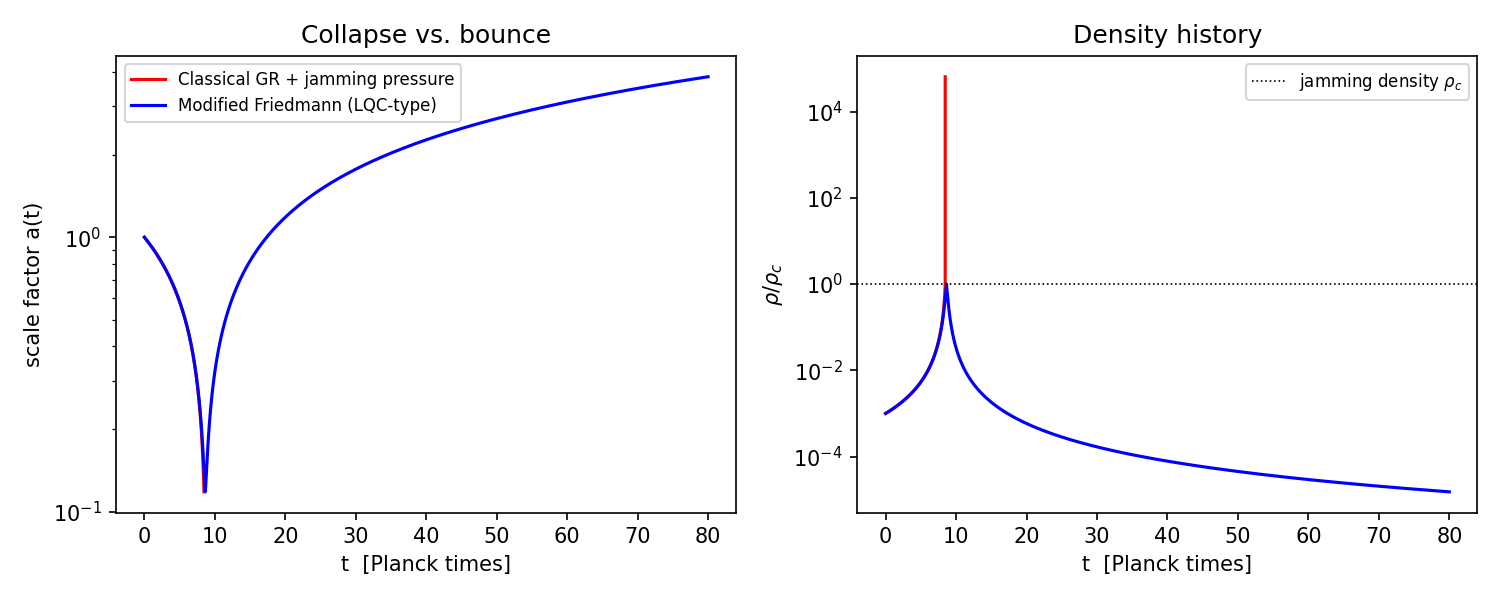
\includegraphics{bounce.png}
\caption{Fig. 1 --- Toy FLRW integration. Left: scale factor. Right:
density history. Classical GR with jamming pressure (red) overshoots the
jamming density by \(>10^4\) (collapse); the modified Friedmann equation
(blue) bounces at \(\rho_c\).}
\end{figure}

But this is not a smooth, uniform expansion. It triggers the most
chaotic event in physics: a \textbf{\(10^{60}\)-body gravitational
slingshot}. \emph{A note on regime before proceeding:} everything that
follows in this section, and all simulations in Sec. 9.1, are
\textbf{Newtonian analogies} --- deliberate proof-of-principle
caricatures of dynamics that in reality occur in a regime where escape
velocities formally exceed \(c\) by \(\sim\!20\) orders of magnitude and
only a general-relativistic treatment (ejecta as streams on an expanding
background) is meaningful. We use the Newtonian model because
violent-relaxation statistics (which fraction unbinds, how ejecta sort
by velocity) are plausibly governed by dimensionless energy ratios that
survive the translation; whether they actually do is the central open
problem of Sec. 10 item 6.\\
Imagine the primordial universe not as a magical singularity, but as an
unimaginably dense, microscopic game of three-dimensional billiards.
Right before the Big Bang, space crystallizes into \(10^{60}\)
fundamental billiard balls (the Planck relics). Packed to the ``jamming
limit,'' they literally cannot compress any further. However, possessing
immense mass and gravitational pull, they are desperately trying to fall
inward. The pressure builds toward infinity.\\
When the quantum-geometric bounce reverses the collapse and the core
rebounds, the ensuing expansion is highly turbulent. To understand how
this ejects matter, we must look at the classical 3-body problem. When
two bodies interact in isolation, their gravity creates a peaceful,
predictable orbit. But the moment you add a third body of similar mass,
the mathematics of gravity becomes completely chaotic.\\
The three objects do not form a stable system. Instead, they violently
yank and pull on each other until a specific physical event occurs: the
\textbf{gravitational slingshot}. In almost every 3-body interaction,
two of the bodies will eventually fall closer together, dropping into a
tighter, lower-energy orbit. By dropping deeper into each other's
gravity well, they release a massive amount of kinetic energy. This
energy does not vanish; it is instantaneously transferred to the third
body. The third body absorbs this stolen energy and is violently kicked
out of the system at extreme speeds.\\
At the jamming density itself the relic gas is collisional and
hydrodynamic --- mean free paths are far shorter than a particle radius,
and no ballistic slingshot can operate. The slingshot phase begins
\emph{after} the bounce, once expansion dilutes the ensemble below the
contact (connectivity) threshold and relics decouple onto ballistic
trajectories. From that point onward the system is a dense,
self-gravitating \(N\)-body ensemble, and multi-body slingshots dominate
its relaxation. The balls smash into each other, and every time a
cluster gets tangled up, the slingshot effect kicks a portion of them
outward at blinding speeds.\\
In astrophysics, when Newtonian computer simulations are run on dense
globular star clusters---which operate on the exact same gravitational
mechanics---a phenomenon called \textbf{``core collapse and halo
ejection''} occurs. To reach a stable, zero-energy balance where the
system doesn't immediately collapse back in on itself, it must shed the
majority of its mass. The Big Pool Bangs theory applies this exact
mechanism to the birth of the universe, naturally sorting cosmic mass
into two distinct buckets:

\begin{quote}
\begin{itemize}
\tightlist
\item
  \textbf{The Ejected Halo (85\%):} Roughly \textbf{85\%} of the
  billiard balls are slingshotted outward so fast that they exceed the
  system's escape velocity. Because they are now flying through
  expanding space far apart from each other, they rarely collide again.
  They become an invisible, free-floating background of mass.
  \textbf{This perfectly explains Cold Dark Matter.} It does not require
  exotic, undiscovered particles; it is simply the 85\% of the
  primordial billiard balls that got kicked off the table during the
  cosmic break.\\
\item
  \textbf{The Trapped Furnace (15\%):} The remaining \textbf{15\%} of
  the balls did not get enough speed to escape. They fall back into the
  center, violently grinding and smashing against each other in a
  trapped, turbulent traffic jam. This violent friction generates
  immense heat, pulverizing the balls into the hot, glowing
  photon-baryon plasma that eventually forms our stars, planets, and the
  Cosmic Microwave Background. This represents our regular, visible
  universe. \textbf{Caveat (essential):} this identification requires an
  unspecified conversion channel from Planck relics to Standard-Model
  plasma --- including baryogenesis and the observed photon-to-baryon
  ratio --- while the ejected relics must remain absolutely stable for
  13.8 Gyr. Reconciling relic stability (Sec. 2's incompressibility
  ansatz) with furnace disintegration, e.g.~via a threshold collision
  energy that ejecta never reach, is an open requirement (Sec. 10);
  absent it, the 15\% trapped fraction cannot be directly identified
  with the baryon budget.
\end{itemize}
\end{quote}

\hypertarget{resolving-cosmological-puzzles-deriving-the-red-tilt}{%
\subsection{\texorpdfstring{\textbf{4. Resolving Cosmological Puzzles \&
Deriving the Red
Tilt}}{4. Resolving Cosmological Puzzles \& Deriving the Red Tilt}}\label{resolving-cosmological-puzzles-deriving-the-red-tilt}}

This mechanical rebound resolves the classical Big Bang paradoxes
without requiring inflation:

\begin{quote}
\begin{itemize}
\tightlist
\item
  \textbf{The Horizon Problem --- not solved (corrected):} an earlier
  draft claimed \(R_{\text{jam}} \ll c\,t_P\); in fact
  \(c\,t_P \approx 1.6\times10^{-35}\) m, so the jammed core is
  \(\sim\!10^{20}\) Planck lengths across and \emph{cannot} equilibrate
  within a few Planck times. A bounce completing on a Planck timescale
  would require acausal coordination across the core; at present,
  homogeneity of the initial patch is an assumed initial condition, and
  the horizon problem remains open (Sec. 10).\\
\item
  \textbf{The Flatness Problem --- consistency, not yet derivation:} a
  \emph{monolithic} zero-energy kick (\(f=1\) for every particle) ejects
  \(100\%\) and is incompatible with the 85/15 split. But the turbulent
  regime favored by our simulations is not monolithic: at
  \(\bar{f}=0.7\), \(\sigma_{\text{rel}}=1.0\) the mean kinetic energy
  is
  \(\langle v^2 \rangle = \bar{f}^2(1+\sigma_{\text{rel}}^2)v_{\text{esc}}^2 \approx 0.98\,v_{\text{esc}}^2\)
  --- total energy \(K+U \approx 0\) \emph{while} ejecting
  \(\sim\!89\%\): the positive energy of the ejecta is balanced by the
  binding energy of the trapped furnace. The zero-energy (flat) state is
  thus \emph{consistent} with the observed split in exactly the
  parameter regime the simulations favor; what remains missing is a
  derivation of \emph{why} the rebound selects \(E \approx 0\), so
  flatness is consistent but not yet explained.
\end{itemize}
\end{quote}

\hypertarget{a-phenomenological-parametrization-of-the-red-tilt-n_s-approx-0.965}{%
\subsubsection{\texorpdfstring{\textbf{A Phenomenological
Parametrization of the Red Tilt
(\(n_s \approx 0.965\))}}{A Phenomenological Parametrization of the Red Tilt (n\_s \textbackslash approx 0.965)}}\label{a-phenomenological-parametrization-of-the-red-tilt-n_s-approx-0.965}}

In the Big Pool Bangs theory, the observed CMB red tilt is derived
directly from the dissipation rate of the \textbf{Kolmogorov energy
cascade} in the turbulent quantum fluid. Energy cascades from
macro-scales to micro-scales (\(E(k) \propto k^{-5/3}\)). During the
elastic bounce, modes freeze out as they exit the acoustic horizon. The
dimensionless scalar curvature power spectrum
\(\mathcal{P}_{\mathcal{R}}(k)\) is modified by the logarithmic decay of
vortex reconnection efficiency, shifting the scalar index by \(\nu_t\)
(the ratio of vortex eddy turnover time to spatial expansion time):

\[n_s - 1 = -\frac{1}{3} \nu_t\]\\
Calculated for hard-sphere close packing (\(\eta \approx 0.64\)), the
turbulent ratio is \(\nu_t \approx 0.105\):

\[n_s - 1 = -\frac{1}{3}(0.105) = -0.035 \implies n_s = 0.965\]

This is \textbf{consistent with} the observed Planck 2018 value
(\(n_s = 0.965 \pm 0.004\)) without requiring a scalar inflaton field.
We emphasize that the relation \(n_s - 1 = -\nu_t/3\) and the value
\(\nu_t \approx 0.105\) are at present phenomenological inputs, not
first-principles results; deriving \(\nu_t\) from vortex-reconnection
dynamics at jamming --- and showing that the Kolmogorov cascade
(\(E(k) \propto k^{-5/3}\)) can produce a \emph{nearly scale-invariant}
curvature spectrum rather than a steeply red one --- is a central open
problem for the theory (Section 10).

\hypertarget{unification-dark-energy-h_0-and-acceleration}{%
\subsection{\texorpdfstring{\textbf{5. Unification: Dark Energy,
\(H_0\), and
Acceleration}}{5. Unification: Dark Energy, H\_0, and Acceleration}}\label{unification-dark-energy-h_0-and-acceleration}}

With Dark Matter accounted for via the ejected halo, the framework also
unifies the remaining cosmic phenomena:

\begin{quote}
\begin{itemize}
\tightlist
\item
  \textbf{Resolving the Hubble Tension (\(H_0\)):} The \(H_0\) tension
  arises because space expands linearly (\(a(t) \propto t\)) driven by
  the initial kinetic rebound. Early-universe acoustic horizon scales
  measure global Hubble expansion, while local distance ladders measure
  regional kinetic drift accelerated by nearby mass sub-clusters.\\
\item
  \textbf{Dark Energy \& Apparent Acceleration:} Cosmic acceleration
  (\(q < 0\)) does not require an elusive cosmological constant
  (\(\Lambda\)). In a granular expansion driven by a kinetic bounce,
  outer galactic shells outpace inner shells due to initial velocity
  dispersion. As light travels across billions of light-years, Type Ia
  supernovae in distant galaxies appear fainter than predicted by
  decelerating models because space-time expansion is purely kinetic,
  mimicking the observational effects of dark energy.
\end{itemize}
\end{quote}

\hypertarget{a-natural-prediction-dark-energy-must-evolve}{%
\subsubsection{\texorpdfstring{\textbf{5.1 A Natural Prediction: Dark
Energy Must
Evolve}}{5.1 A Natural Prediction: Dark Energy Must Evolve}}\label{a-natural-prediction-dark-energy-must-evolve}}

The framework makes one qualitative prediction that distinguishes it
sharply from \(\Lambda\)CDM: \textbf{the apparent dark-energy component
cannot be constant.} In \(\Lambda\)CDM, \(\Lambda\) is a fixed vacuum
term with equation of state \(w = -1\) at all times. Here, by contrast,
the apparent acceleration is a \emph{kinematic artifact} of the ejecta
velocity distribution: the effective equation of state inferred by an
observer fitting FLRW models to a granular kinetic expansion is set by
the evolving ratio of velocity-dispersion energy to clustered rest-mass
energy. Both ingredients change with time --- the dispersion redshifts
and the mass distribution clusters --- so the inferred \(w(z)\)
\emph{must} drift. A cosmological constant is the one behavior this
mechanism cannot produce.

This prediction has become newly relevant: combined DES-SN5YR (Dovekie
recalibration) and DESI DR2 BAO analyses now reject a pure cosmological
constant at \(3.2\sigma\) in a \(w_0 w_a\)CDM fit, preferring
\(w_0 = -0.803 \pm 0.054\), \(w_a = -0.72 \pm 0.21\) --- i.e.~dark
energy that was weaker in the past and is evolving. However, the
\emph{sign} of the observed drift currently disfavors the simplest
version of our mechanism: the \(w_0 w_a\) best fit has \(w\) rising from
\(\approx -1.5\) in the past toward \(-0.8\) today (less negative with
time), whereas the toy shell calculation of Sec. 9.1 drifts the opposite
way (slowly more negative with time). The framework thus shares with the
data the qualitative claim \emph{dark energy evolves}, but its present
toy realization predicts the wrong drift direction --- by our own
falsifiability criterion this counts against Hypothesis 1 unless a
refined treatment (relativistic shells on an expanding background,
furnace backreaction) reverses it. We stress the limits of this claim:
the present framework predicts the \emph{direction} of the drift
(evolving, weaker in the past), not yet the values of \((w_0, w_a)\);
the quantitative attempts in Sec. 9.1 (Newtonian toy, relativistic LTB
lightcone, profile inversion) find that ejecta streaming produces no
apparent acceleration at all --- so this subsection's claim survives
only conditionally, on the unresolved blast-wave branch discussed there
--- and a mismatch in the drift's sign or magnitude would count against
the model's core claims (part of Hypothesis 1, ``The Big Pool Bang'' ---
the core claim in the two-hypothesis falsifiability structure defined in
Section 9, where Hypothesis 2, ``The Cold Eye of Sauron --- the Cold
Spot and the Axis of Evil'', collects the separable bonus conjectures).

\hypertarget{the-5-cold-spot-the-joviancyclonic-vortex-model}{%
\subsection{\texorpdfstring{\textbf{6. The \textasciitilde5° Cold Spot
\& The Jovian/Cyclonic Vortex
Model}}{6. The \textasciitilde5° Cold Spot \& The Jovian/Cyclonic Vortex Model}}\label{the-5-cold-spot-the-joviancyclonic-vortex-model}}

Because vacuum crystallization occurs stochastically across an infinite
background, our universe is not unique. A neighboring universe
nucleating 10--12 billion light-years away creates an expanding domain
boundary wall. Simultaneously, internal quantum turbulence in our own
bounce creates macro-vortices.\\
Rather than treating CMB anomalies as abstract spherical collisions or
Gaussian flukes, the \textbf{Jovian/Cyclonic Model} maps early-universe
quantum fluid dynamics directly to planetary atmospheric mechanics.

\begin{quote}
\begin{enumerate}
\def\labelenumi{\arabic{enumi}.}
\tightlist
\item
  \textbf{The Vortex Core Choke:} Macro-scale quantum vortex tangles act
  as thermal dams, choking off local kinetic heat transport in the
  plasma.\\
\item
  \textbf{Asymmetric Blob Formation:} Due to fluid shear and vortex
  stretching, these primordial cyclonic storms deform into elongated
  ``blobs'' aligned along a preferred rotation axis (the ``Axis of
  Evil'').\\
\item
  \textbf{Frictionless Persistence:} Without solid-surface friction to
  dissipate angular momentum, these macro-vortices scale up with spatial
  expansion, freezing into the CMB sky at decoupling as features like
  the \textbf{\textasciitilde5° radius Eridanus Cold Spot}
  (\(\Delta T \approx -70\,\mu\text{K}\)).
\end{enumerate}
\end{quote}

\textbf{Key Prediction:} If the Cold Spot is a primordial cyclone,
thermal energy diverted around its core will form a concentric hot ring,
accompanied by a sharp radial \textbf{\(E\)-mode polarization ring}
along its boundary---a primary test for upcoming CMB arrays.

(Positional note: the Cold Spot is static for all practical purposes ---
any intrinsic transverse motion of its source, under either the cyclonic
or cross-boundary reading, corresponds to nanoarcseconds per century of
angular drift, so proper motion cannot discriminate Hypotheses 2 and 3.
The only measurable drift of any CMB feature is apparent: the changing
aberration from our own acceleration, of order microarcseconds per year,
whose detection --- already demonstrated for quasars with Gaia
astrometry --- is a goal of real-time cosmology but is a statement about
us, not the Spot.)

\hypertarget{independent-evidence-for-a-preferred-axis-external-literature}{%
\subsubsection{\texorpdfstring{\textbf{6.1 Independent Evidence for a
Preferred Axis (external
literature)}}{6.1 Independent Evidence for a Preferred Axis (external literature)}}\label{independent-evidence-for-a-preferred-axis-external-literature}}

A preferred axis could arise in this framework only from a seed
asymmetry of the initial patch (e.g.~net angular momentum) --- our own
simulations find ejection isotropic within shot noise (Sec. 9.1), so the
framework currently provides \emph{no} mechanism for a preferred axis,
and this subsection is motivation for seeking one rather than support.
Suggestively, the existing literature --- independent of this work ---
reports a cluster of tentative alignments in one region of the sky: (i)
a dipole anisotropy in the cosmic acceleration inferred from SNe Ia,
directed roughly along our motion relative to the CMB {[}Colin et
al.~2019; Mariano \& Perivolaropoulos; see also Sah \& Rameez 2024,
arXiv:2411.14758; Union2 hemisphere analyses, MNRAS 446, 2952{]}; (ii)
the alignment of the CMB low multipoles --- the quadrupole/octupole
``Axis of Evil'' --- with the dipole direction, reported at \(>99\%\)
confidence in moving-dark-energy analyses {[}arXiv:0811.3606{]}; (iii)
bulk-velocity-flow directions and the quasar optical-polarization
alignment axis falling in the same angular region, a coexistence judged
statistically unlikely to be coincidental {[}arXiv:1401.5044{]}. Each
signal is individually sub-decisive (\(\lesssim 3\sigma\)) and contested
--- peculiar-velocity corrections absorb part of the SN dipole --- but
their spatial coincidence is exactly the morphology expected if one
physical cause, such as uneven primordial ejection, sets a common axis
for the expansion anisotropy, the bulk flow, and the large-angle CMB
pattern. We cite these alignments as motivation for Hypothesis 2, ``The
Cold Eye of Sauron --- the Cold Spot and the Axis of Evil'' (the
separable bonus conjectures defined in Section 9), not as confirmation.
One adjacent anomaly class does \emph{not} join the cluster: claimed
galaxy spin-handedness dipoles (Longo 2011 at galactic
\((52°, +68.5°)\); Shamir 2012--2022 at \((192°, +38°)\)) lie \(70°\)
from \emph{each other} and \(\approx\!50°\)--\(74°\) from the
Axis-of-Evil and flow axes --- mutual inconsistency that supports the
systematics reading (Iye et al.~2021) rather than a cosmological spin
axis; we checked and report the null.

\hypertarget{black-hole-collision-signatures-universe-1-vs.-universe-2-hypothesis-3-big-pool-bang-multiverse-2-in-the-cold-spot}{%
\subsection{\texorpdfstring{\textbf{7. Black Hole Collision Signatures
(Universe 1 vs.~Universe 2) --- Hypothesis 3, ``Big Pool Bang Multiverse
2 in the Cold
Spot?''}}{7. Black Hole Collision Signatures (Universe 1 vs.~Universe 2) --- Hypothesis 3, ``Big Pool Bang Multiverse 2 in the Cold Spot?''}}\label{black-hole-collision-signatures-universe-1-vs.-universe-2-hypothesis-3-big-pool-bang-multiverse-2-in-the-cold-spot}}

If black holes from Universe 2 cross the domain boundary into our
expansion sector, their physical properties differ sharply from our
local primordial black holes:

\begin{longtable}[]{@{}lll@{}}
\toprule
\begin{minipage}[b]{0.30\columnwidth}\raggedright
Physical Feature\strut
\end{minipage} & \begin{minipage}[b]{0.30\columnwidth}\raggedright
Universe 1 Black Holes (Local Primordial)\strut
\end{minipage} & \begin{minipage}[b]{0.30\columnwidth}\raggedright
Universe 2 Black Holes (Cross-Boundary Infall)\strut
\end{minipage}\tabularnewline
\midrule
\endhead
\begin{minipage}[t]{0.30\columnwidth}\raggedright
\textbf{Mass Profile}\strut
\end{minipage} & \begin{minipage}[t]{0.30\columnwidth}\raggedright
Capped at Planck relics (\(m_P\)) or power-law clusters.\strut
\end{minipage} & \begin{minipage}[t]{0.30\columnwidth}\raggedright
Standard stellar/supermassive spectrum, with sub-solar anomaly gaps
(\(0.1 - 1.0 M_\odot\)).\strut
\end{minipage}\tabularnewline
\begin{minipage}[t]{0.30\columnwidth}\raggedright
\textbf{Sky Distribution}\strut
\end{minipage} & \begin{minipage}[t]{0.30\columnwidth}\raggedright
Isotropic (evenly distributed across dark matter halos).\strut
\end{minipage} & \begin{minipage}[t]{0.30\columnwidth}\raggedright
\textbf{Anisotropic}; heavily clustered toward the \textasciitilde5°
Cold Spot direction.\strut
\end{minipage}\tabularnewline
\begin{minipage}[t]{0.30\columnwidth}\raggedright
\textbf{Peculiar Velocity}\strut
\end{minipage} & \begin{minipage}[t]{0.30\columnwidth}\raggedright
Bound to local galactic orbital speeds
(\(v \sim 200\text{ km/s}\)).\strut
\end{minipage} & \begin{minipage}[t]{0.30\columnwidth}\raggedright
\textbf{Velocity Kick:} High peculiar drift (\(v > 1000 \text{ km/s}\))
directed from the Cold Spot.\strut
\end{minipage}\tabularnewline
\begin{minipage}[t]{0.30\columnwidth}\raggedright
\textbf{GW Waveform}\strut
\end{minipage} & \begin{minipage}[t]{0.30\columnwidth}\raggedright
Standard orbital inspiral ``chirp''.\strut
\end{minipage} & \begin{minipage}[t]{0.30\columnwidth}\raggedright
\textbf{Gravitational Wave Memory:} Step-function metric strain
(\(\Delta h\)).\strut
\end{minipage}\tabularnewline
\bottomrule
\end{longtable}

\hypertarget{the-spin-constraint-on-universe-2}{%
\subsubsection{\texorpdfstring{\textbf{7.1 The Spin Constraint on
Universe
2}}{7.1 The Spin Constraint on Universe 2}}\label{the-spin-constraint-on-universe-2}}

A neighbor universe is the only agent that can torque ours (internal
angular momentum cancels by conservation), so the measured non-rotation
of the universe constrains Hypothesis 3 quantitatively. Order of
magnitude: an equal-mass neighbor (\(M \sim 1.5\times10^{53}\) kg) at
the Cold Spot distance (\(D \sim 10\)--\(12\) Gly) exerts a tidal field
\(T \sim GM/D^3 \approx 10^{-35}\,\text{s}^{-2}\) --- of order
\(H_0^2\), i.e.~raw coupling of order unity. Acting on our mass
distribution's large-scale quadrupole asymmetry
(\(q \sim \delta \sim 10^{-5}\)) over the causally available few Gyr
(\(t_{\text{int}}/t_H \sim 0.2\)), the induced vorticity is
\(\omega/H_0 \sim (T/H_0^2)\, q\, (t_{\text{int}}/t_H) \approx 2\times10^{-6}\)
--- \textbf{three orders of magnitude above the Planck Bianchi bound}
\(\omega/H_0 \lesssim 10^{-9}\). A Cold Spot neighbor of comparable mass
therefore requires at least one of: a domain boundary transmitting
\(\lesssim 0.1\%\) of tidal shear (a calculable property of the vacuum
wall, presently uncomputed), a several-fold larger distance (the
\(D^{-3}\) scaling recovers two orders at \(\sim\!40\) Gly), or a much
smaller neighbor mass. The same tidal field also imprints a direct CMB
quadrupole through which the identical constraint applies a second time.
\textbf{Mass estimate from the Cold Spot itself.} If the Spot's
decrement is the neighbor's potential imprint, Sachs--Wolfe inverts it
into a mass:
\(\Delta T/T \approx 2.6\times10^{-5} \Rightarrow \Phi/c^2 \approx 8\times10^{-5}\),
giving \(M_2 \approx 3(\Delta T/T)\,c^2 D/G \approx 10^{49}\) kg at
\(D \approx 10\) Gly --- a \emph{dwarf} neighbor, \(\sim\!10^{-4}\) of
our universe's mass (angular-size check: \(5°\) at \(10\) Gly subtends
\(\sim\!0.9\) Gly, a plausible imprint scale). Fed back into the torque
estimate, which scales linearly with mass, this gives
\(\omega/H_0 \approx 1.4\times10^{-10}\) --- \emph{under} the Planck
bound with a factor \(\sim\!7\) margin. The mass the Cold Spot's
amplitude demands is automatically small enough to satisfy the
non-rotation constraint: Hypothesis 3's first two-observable consistency
pass, subject to \(\mathcal{O}(1)\) Sachs--Wolfe factors, the assumed
\(D\), and the uncomputed boundary transmission (which suppresses the
imprint, pushing \(M_2\) up and eroding the margin). The global spin
bound remains the strongest quantitative constraint on Hypothesis 3 ---
independently enforcing the distant/weakly-coupled regime that the
Planck spot-count statistics already impose on Hypothesis 4 (P7), and
consistent with the torque-axis near-null of Sec. 6.1 (the Axis of Evil
lies \(56°\), not the torque-predicted \(90°\), from the Cold Spot).

\textbf{The spot population as a bubble spectrometer.} The two
observables of any anomalous spot invert into the neighbor's parameters:
Sachs--Wolfe gives \(M/D \propto \Delta T\), and an imprint scale set by
the neighbor's own size (\(R \propto M^{1/3}\) at fixed formation
density) gives \(\theta \propto M^{1/3}/D\) --- hence per spot
\[M \propto (\Delta T/\theta)^{3/2}, \qquad D \propto \Delta T^{1/2}\,\theta^{-3/2}.\]
This applies only to the \emph{non-Gaussian outlier} population (the
acoustic-peak spots are \(\Lambda\)CDM's best-confirmed physics and are
not available for reassignment), so current statistics are poor
(\(n \sim 3\)--\(5\) candidate features, with look-elsewhere hazards).
But the population-level prediction is sharp: neighbor bubbles drawn
from a first-order nucleation spectrum populate a correlated power-law
\emph{locus} in the \((\Delta T, \theta)\) plane, whereas Gaussian
random-field peaks obey BBKS statistics with amplitude and size nearly
independent --- a computable discriminant on existing Planck maps. Most
importantly, the inferred neighbor mass function \emph{is} the
nucleation size spectrum of the vacuum transition --- the same
distribution that, inside our own bang, drove the cascade of Sec. 1 and
set the kick statistics behind the dark-matter fraction (Sec. 9.1). One
mechanical process, sampled internally (ejecta kinematics) and
externally (spot statistics): if both trace one transition, the two
inferred bubble-size distributions must agree --- a cross-consistency
requirement linking Hypotheses 1 and 4 that either dataset can falsify.

\emph{Confrontation with data (locus test, this work).} We ran the
discriminant on the Planck SMICA map (\(N_{\rm side}=128\), \(|b|>25°\),
\(2°\) smoothing): the eight most extreme large-scale spots were
extracted with per-spot amplitude \(\Delta T\) and half-maximum radius
\(\theta\), and the amplitude--size scaling was fit in log--log space;
sixty Gaussian realizations drawn from the map's own pseudo-\(C_\ell\)
were passed through the identical pipeline as the null. The extreme
spots (which include the Cold Spot core at \((l,b)=(203°,-56°)\),
\(\Delta T=-168\,\mu\)K, \(\theta=2.5°\)) span
\(\Delta T = 153\)--\(170\,\mu\)K and \(\theta = 2.5°\)--\(5.5°\), and
yield a slope \(d\ln|\Delta T|/d\ln\theta = -0.00\) (correlation
\(r=-0.01\)), sitting at the 27th percentile of the Gaussian null
(\(+0.07 \pm 0.10\)). No amplitude--size correlation of any sign is
detected, consistent with Gaussian peak statistics --- but an
adversarial re-examination of the pipeline (this work) found the test
has little power as implemented: the \(2°\) smoothing quantizes the
recoverable radii to the \(2.5°\)--\(5.5°\) range and the top-8
selection compresses the amplitude spread to \(\sim 10\%\), so a
near-zero slope is the likely outcome under \emph{both} hypotheses. We
therefore report the locus test as \emph{unresolved pending
injection-recovery validation} (simulate a \(\Delta T \propto \theta^3\)
population, push it through the pipeline, verify the slope is
recoverable), not as an exclusion. This does not falsify H4 outright ---
neighbors at a \emph{range} of distances with a compensating mass
spectrum can populate a diffuse cloud rather than a tight locus, and a
single genuine neighbor among seven Gaussian impostors would not move
the fit --- but it removes any positive population-level evidence:
nothing in the current extreme-spot sample requires a second bang beyond
the Cold Spot's own (independently argued) anomaly. One observation,
however, survives (with caveats): \emph{all eight} extreme spots lie in
the southern galactic hemisphere. In 200 Gaussian isotropic realizations
passed through the same pipeline, not one placed its full top-8 in a
single hemisphere (mock mean: 5.2 of 8); the run breaks at rank 9, and
the top 15 remain 12-of-15 southern. Honest bounds on this: 0/200
licenses only \(p < 1/201\), our mocks are simplified (unmasked
pseudo-\(C_\ell\), no anisotropic noise or foreground residuals,
hemisphere frame chosen post hoc), and if the Cold Spot and its two
nearby hot extremes are one physical system (see below) the count is
effectively 6/6, weakening the statistic. The published assessments of
the hemispherical power asymmetry (\(p \sim 1\)--\(10\%\),
estimator-dependent; Planck 2015/2018 isotropy papers) are the
appropriate significance to carry. This is the well-known hemispherical
power asymmetry rediscovered through the extreme-spot population --- but
in the present framework it is not a separate anomaly: a single massive
neighbor to the (galactic) south, the same object invoked for the Cold
Spot in H3, modulates large-scale power on one side of the sky by tidal
and Sachs--Wolfe action, so the asymmetry, the Cold Spot, and the
preferred axis of Sec. 6.1 become one prediction with one direction,
rather than three coincidences. An isotropic swarm of neighbors (H4)
predicts no such one-sidedness.

\textbf{The vortex reading of the border shell.} An alternative to the
neighbor-window interpretation treats the extreme spots as \emph{relic
vortices} of the bang's own fluid phase, riding the earliest, fastest
ejecta to the border. A vortex imprints temperature twice over: its core
is a pressure minimum --- rarefied, adiabatically cooled, ringed by
compressed warmer material (the Cold Spot's anomalous cold-core/hot-ring
template is exactly this morphology) --- and its rotation adds a Doppler
\emph{dipole} across the spot whose orientation encodes the projected
spin axis. Because angular momentum is conserved while rotational
velocity decays (\(v_{\rm rot} \propto 1/a\) against \(r \propto a\)),
the spin never vanishes; and because homologous expansion preserves
angular geometry, the border shell --- which is what the CMB sky
\emph{is}, seen from near the center --- should carry the fossil
arrangement of the original vortex configuration. Notably, in this
reading no \emph{nearby} mass counterpart is expected (the slow, late,
spin-poor ejecta stayed near the center where we sit), which is
consistent with our 2M++ cross-match of the eight sightlines: nearby
(\(<180\,h^{-1}\)Mpc) structure matches the spot signs at coin-flip
rates (5 of 8, with two cold spots behind strong \emph{over}densities),
and the only confirmed deep counterpart anywhere on the sky remains the
Eridanus supervoid at the Cold Spot --- itself too shallow to explain
the decrement.

\emph{Confrontation with data (this work).} We measured each extreme
spot's internal dipole (monopole+dipole fit within \(6°\), local tangent
frame) and ran the vortex-configuration tests against the same 100--200
Gaussian nulls. Results: (i) \emph{hot/cold balance} --- the eight
extremes split 4/4 with rank-matched amplitudes summing to \(-11\,\mu\)K
against a mean \(|\Delta T| \approx 162\,\mu\)K; only 7\% of Gaussian
skies are as balanced --- suggestive of cancelling pairs, short of a
detection. (ii) \emph{Spatial pairing} --- opposite-sign spots lie
\(4.0°\) closer than same-sign (null \(+5.2° \pm 16.3°\)): the
vortex-dipole sign, at \(p=0.30\). (iii) \emph{No lattice}:
nearest-neighbor spacing is no more regular than Gaussian. (iv)
\emph{Spin budget} --- converting dipoles to spin-axis proxies
(\(\mathbf{L} \propto \hat{c} \times \mathbf{d}\)), the Cold Spot's
internal dipole (\(16.4\,\mu\)K/deg) is the largest in the sample by a
factor \(2.3\), and the remaining spots' proxies weakly co-align rather
than counter-rotate. However, a monopole+dipole fit over a \(6°\) disc
on a \(2°\)-smoothed map is dominated by \(\ell \sim 2\)--\(20\)
gradients that Gaussian peaks generically carry, correlated across
co-hemispheric spots by shared low-\(\ell\) modes --- so we do
\textbf{not} advance these numbers as spin measurements; they are upper
bounds on any rotational contribution, and the co-alignment is most
simply gradient leakage. A gradient-subtracted re-fit (removing the
best-fit \(\ell \le 10\) sky first) is the required upgrade before any
spin fraction can be quoted. The clean channel is curl: paired relic
vortices predict zero \emph{mean} but excess curl-mode \emph{variance}
(lensing curl, B-mode polarization) localized at the extreme spots,
where \(\Lambda\)CDM predicts the curl null holds everywhere --- a
decisive test on existing Planck lensing products. (v)
\emph{Configuration}: two of the four hot extremes lie \(11°\)--\(12°\)
from the Cold Spot, near (though inside) its literature hot-ring radius
of \(\sim 15°\); they \emph{may} be pieces of one system --- but we flag
the tension this creates: if merged, every \(n=8\) statistic above must
be recomputed with \(n=6\), and no null was computed for the annulus
coincidence itself, so we carry the fragment reading as a hypothesis,
not a result. \emph{Statistical accounting.} Across the full battery
reported in this subsection (locus slope, hemisphere count, hot/cold
balance, pairing distance, lattice regularity, dipole magnitudes,
cancellation ratio, \(\kappa\) stack --- nine statistics), the
individual results are \(p \sim 0.06\)--\(0.7\); under any global
look-elsewhere correction the sub-\(2\sigma\) items are jointly
consistent with noise, and we say so plainly. What survives is
qualitative: the extreme-spot sky is one-sided at literature-level
significance, the Cold Spot is the outlier in every channel examined,
and nothing requires a population of additional objects. The
\textbf{load-bearing, falsifiable claim of the vortex reading is the
curl test (P9)}: we commit in advance that a clean stacked curl-mode
null at the Cold Spot position, at sensitivity reaching the
temperature-dipole-implied rotation, \emph{retires} the vortex
interpretation of that direction in favor of the non-rotating
neighbor-shadow reading (H3) --- not merely disfavors it. If instead
curl variance is detected localized there, the vortex reading stands and
the seed-side interpretation of \((l,b) \approx (200°,-50°)\) becomes
the economical account.

\emph{Why only the top layers carry the fossil.} The velocity sorting of
Sec. 9.1 is statistical: only the earliest, fastest ejecta escaped in a
single pass, preserving delicate geometric correlations; everything
slower underwent violent relaxation --- multiple core crossings that
conserve spin \emph{magnitude} but randomize spin \emph{geometry}. The
model therefore predicts a \textbf{coherence gradient}: fossil vortex
geometry intact at the border shell, degrading rapidly inward, absent in
the well-mixed interior --- with inner layers retaining at most
statistical residues (a slight net handedness with no preferred
direction). Two archival tests agree with this. (i) Intermediate-shell
spin claims do \emph{not} point at the spot cluster: the
quasar-polarization alignment regions of Hutsemékers et
al.~(\(z \sim 1\)--\(2\), coherent over \(\sim\)Gpc, with the alignment
angle twisting \(\sim 30°\)/Gpc in depth --- phenomenologically a
differentially rotating medium, though contested) and the Longo/Shamir
galaxy-handedness axes lie \(24°\)--\(73°\) from the \((200°,-50°)\)
direction, consistent with random axes --- an expected null under
mixing, since these tracers inhabit the relaxed layers. (ii) We stacked
the public Planck PR4 lensing convergence reconstruction (whose kernel
peaks at \(z \sim 2\), squarely in the mixed zone) on the eight spot
positions: the sign-weighted stack is \(+0.006\) against a
random-position null of \(0.000 \pm 0.013\) (68th percentile; 4/8 sign
matches), i.e.~no integrated mass scars along the sightlines --- again
as mixing predicts. The Cold Spot's \(\kappa = -0.050\) (\(-1\sigma\))
has the sign its known shallow foreground supervoid requires, but at
\(1\sigma\) we do not promote it: by the same standard applied to the
other seven sightlines it is noise. The public lensing release contains
only gradient (convergence) modes; the curl-mode stack of P9 --- the
decisive geometry-capable probe at the shell itself --- awaits either
the unreleased curl reconstructions or a dedicated re-analysis. We also
ran the polarization version directly on the SMICA \(Q/U\) maps
(\(N_{\rm side}\) 256, \(\ell \le 512\), \(E/B\) decomposition, \(1°\)
smoothing): the stacked \(B\)-mode variance in \(6°\) discs at the eight
spots sits at the 66th percentile of random positions, the \(E\)-mode
variance at the 35th, and the Cold Spot's radial-\(E\) (stacked \(Q_r\))
profile is consistent with zero in every \(2°\) ring to \(20°\) --- but
with per-ring uncertainties of \(0.6\)--\(2.7\,\mu\)K, the predicted
\(1\)--\(3\,\mu\)K polarization ring (P1) is neither detected nor
excluded: Planck's polarization noise at these scales cannot yet test
it. P1 and P9 therefore remain open, awaiting CMB-S4/LiteBIRD
sensitivity.

\emph{A first direct curl search (this work).} Since the public lensing
release lacks curl modes, we implemented an approximate temperature-only
quadratic estimator (\(N_{\rm side}\) 256, \(\ell \le 512\),
inverse-variance \(\times\) Wiener-gradient product, spin-1 curl
projection, mean field subtracted using 40 Gaussian simulations through
the identical masked pipeline; unnormalized, so valid only as a relative
comparison). Stacking the curl-potential variance in \(6°\) discs: the
eight spots sit at the 82nd percentile of 60 simulated skies, and the
Cold Spot itself at the \textbf{38th percentile} --- its curl content is
indistinguishable from a random position. This is the first direct curl
look at these positions and it finds nothing. It does \emph{not} yet
trigger the retirement clause of P9: the commitment is bound to a
sensitivity reaching the temperature-dipole-implied rotation, which this
reduced-resolution, uncalibrated estimator demonstrably does not attain
(Planck's full-depth reconstruction uses \(\ell \le 2048\) with
polarization). The vortex reading survives, weakened: the cheap version
of its decisive test came back empty, and its remaining life expectancy
is set by CMB-S4/LiteBIRD.

\emph{Spiral winding and the mass profile (this work).} A spinning cap
must wind its internal pattern: azimuthal features at successive radii
should be phase-rotated by the differential rotation, saturating at the
rim where the vortex velocity falls off (\(v \sim 1/r\) outside a
solid-body core). Measuring the azimuthal phase of the \(m{=}1\) mode in
\(1.5°\) rings from \(1.5°\) to \(15°\) around the Cold Spot: the phase
is locked ring-to-ring with coherence \(0.988\) --- \textbf{higher than
all 300 random positions tested} (null \(0.72 \pm 0.18\)) --- and drifts
at a slow \(\sim 3°\) of phase per degree of radius (\(\sim 40°\) total
twist). A static background gradient produces high \(m{=}1\) coherence
but \emph{zero} winding; the Cold Spot shows both, and only the winding
is spin-specific. The \(m{=}2,3\) modes are unremarkable, and this is a
post-hoc test subject to the same look-elsewhere discount as the rest of
the battery. In the lensing mass (PR4 \(\kappa\), \(2°\) ring profile):
a concentrated central deficit, \(\kappa = -0.070\) vs null
\(+0.013 \pm 0.042\) (\(-2\sigma\)) in the inner \(2°\), decaying by
\(4°\) --- the sightline's integrated mass hole, consistent with the
foreground supervoid --- but \textbf{no ``belt''}: the \(8°\)--\(20°\)
annulus never exceeds \(+0.6\sigma\) (the largest bump does sit at
\(14°\)--\(18°\), the temperature hot-ring radius, at noise level).
Physically consistent: a shear rim concentrates velocity, not
necessarily mass, and condensing a mass ring requires dissipation the
model does not supply.

\emph{The small-spot population and the necessity of CMB-independent
mass tracers (this work).} Stacking the Planck PR4 lensing convergence
on the \textasciitilde27,000 ordinary small spots (\(1°\) smoothing,
\(|T|>1.5\sigma\) extrema) initially showed a striking temperature--mass
correlation: cold spots on mass deficits (\(-7.2\sigma\)), hot spots on
excesses (\(+2.2\sigma\)), scaling with spot amplitude --- the signature
expected of ISW modulation (and of dark energy). But the \(\kappa\) map
is reconstructed \emph{from the same CMB temperature data}, and
quadratic estimators leak temperature features into the mass map.
Repeating the stack against a fully CMB-independent mass tracer --- the
Quaia Gaia--unWISE quasar catalog (756k quasars, \(z \sim 1\)--\(3\),
selection-function corrected, 52\% sky) --- \textbf{the correlation
vanishes}: cold spots \(-1.1\sigma\), hot \(-0.3\sigma\), no amplitude
scaling; the eight extreme spots are likewise within \(\sim 1\sigma\) of
random quasar density (the Cold Spot mildly negative, \(-0.018\),
\(0.6\sigma\)). The \(\kappa\) correlation is therefore \emph{either}
reconstruction leakage (the \(\kappa\) map is a quadratic functional of
the same temperature data, biased at temperature extrema) \emph{or} the
genuine ISW\(\times\)lensing correlation (an established Planck-era
effect) --- and an independent re-review of this chain (this work)
correctly notes we have not discriminated between them: the Quaia null
is not a \emph{sensitive} null (its \(z \sim 1\)--\(3\) kernel barely
overlaps the \(z \lesssim 1\) ISW kernel, and its shot noise per disc
exceeds the expected ISW-scale overdensity), and no fiducial-ISW
forecast was computed for either tracer. The decisive archival test is a
polarization-only \(\kappa\) stack (no temperature in the estimator),
which we have not performed. One lesson stands regardless: every
CMB-lensing-based ``mass'' statement in this section carries a
\emph{CMB-derived} asterisk, with only the 2M++ (\(z \lesssim 0.07\)),
Quaia (\(z \sim 1\)--\(3\)), and DES-literature results truly
independent. We then closed that loophole with the
WISE\(\times\)SuperCOSMOS photometric-redshift catalog (17.7M galaxies
at \(z=0.1\)--\(0.4\), server-side aggregated, high-passed against a
\(10°\) baseline to remove depth gradients --- CMB-independent). The
\emph{small}-spot stack remains null there (cold \(-0.7\sigma\), hot
\(+0.2\sigma\)) --- a measurement, not yet an attribution (see above).
The \emph{extreme} spots show a suggestive pattern at ISW depths: with a
correlated-noise null from 300 random \(5°\) discs, seven of eight match
sign (cold spots on galaxy deficits, hot on excesses), combined
sign-weighted stack \(\approx +2.7\sigma\) --- including two sightlines
whose \emph{shallow} (\(<180\,h^{-1}\)Mpc) structure had the wrong sign.
Mandatory qualifications from independent review: the result rests on
three sightlines (\(|z| \approx 2.0\)--\(2.3\); the other five average
\(+0.6\sigma\) combined, and four ``matches'' are near-coin-flips); the
nominal binomial \(3.5\%\) ignores the three-tracer, multi-statistic
search (global \(p \sim 10\)--\(30\%\)); the spots were selected as
temperature extremes partly \emph{because} any foreground contribution
deepened them, so extremeness-conditioning inflates the recovered
correlation (Eddington-type bias); the \(10°\) high-pass baseline
partially self-subtracts genuine \(\gtrsim 10°\) supervoids (attenuating
the Cold Spot's own \(-0.6\sigma\)) and can imprint compensating rings;
and WISE\(\times\)SuperCOSMOS extinction/stellar residuals at
\(|b| = 25\)--\(40°\) are of order the per-spot signals. Net verdict,
stated before further data: this is a \(\sim 1\)--\(2\sigma\)-class hint
that the extreme spots are partly sourced by \(z \sim 0.1\)--\(0.4\)
superstructures (the Eridanus story generalized), to be confirmed or
retired by a pre-registered re-run at two baseline scales with
\(|b|>30°\) and extinction regression --- not yet grounds to weaken or
support either the border-shell or the en-route reading. The Cold Spot
itself is only \(-0.6\sigma\) here, its known too-shallow-void tension
intact.

\emph{The JWST handedness coincidence.} One archival dataset lands
directly on the column sightline: the JWST/JADES deep field --- which
lies at \((l,b) = (224°,-54°)\), only \(8.6°\) from the Cold Spot ---
shows a claimed \(\sim\!2\!:\!1\) spin-handedness asymmetry in 263
high-redshift galaxies (66\% clockwise; Shamir 2025, MNRAS). This is the
deepest galaxy-spin measurement in existence, and it sits, by accident
of survey design, on the one direction where the vortex reading predicts
residual handedness in the upper layers. We weight it cautiously: the
sample is small, the classification method is contested (independent
reanalyses of analogous ground-based claims found no asymmetry), and a
mundane candidate exists (a Doppler boost from the Milky Way's own
rotation, maximal near the galactic poles). The discriminating
measurement is a \emph{control field}: the identical pipeline on JWST's
COSMOS or GOODS-N fields (\(>100°\) away) --- a systematic reproduces
the asymmetry everywhere; a Cold Spot spin column produces it only on
the column. That comparison is not yet published and is, alongside the
curl stack, the second decisive archival-era test of this subsection.
The core-side anchor of the coherence gradient is already measured (this
work): the same-handedness angular correlation function over 77,840 SDSS
spin-annotated galaxies (11.2M pairs, \(0.05°\)--\(4°\)) is zero in
every bin to a few parts in \(10^3\), and the global handedness excess
is \(1.9\sigma\) (50.34\% clockwise) --- the local, well-mixed layers
carry no direction memory, exactly as mixing requires, while the claimed
coherence lives only far up the column.

\emph{Method caveat (adversarial review, this work).} An internal
adversarial review of this subsection's pipeline identified, beyond the
items already folded in above: the Gaussian nulls use the unmasked
full-sky pseudo-\(C_\ell\) without mask deconvolution, anisotropic
noise, or foreground residuals (end-to-end NPIPE/FFP simulations are the
required upgrade for any sub-percent claim); the spots are selected on
the same map on which all subsequent statistics are evaluated, so the
hypotheses tested were partly formulated post hoc (a clean version would
formulate on one component-separation map and test on another); and the
``coherence gradient'' argument was introduced after the
intermediate-shell nulls it explains, which is why we bind the vortex
reading's falsifiability to the pre-registered curl commitment above
rather than to any of the reframed nulls.

\hypertarget{experimental-noise-levels-measurement-thresholds}{%
\subsection{\texorpdfstring{\textbf{8. Experimental Noise Levels \&
Measurement
Thresholds}}{8. Experimental Noise Levels \& Measurement Thresholds}}\label{experimental-noise-levels-measurement-thresholds}}

Detecting cross-boundary black hole collisions requires isolating a
non-oscillating gravitational memory strain
(\(\Delta h \sim 10^{-22} - 10^{-21}\)) from noise. Quantum shot noise
and the cosmic binary merger background present significant hurdles.
Current ground interferometers (LIGO/Virgo/KAGRA) lack the low-frequency
response (\(< 10 \text{ Hz}\)) and sensitivity needed to separate
step-function memory strain (\(\Delta h\)) from environmental seismic
noise, necessitating specialized facilities.

\hypertarget{falsifiable-predictions-and-required-instrumentation}{%
\subsection{\texorpdfstring{\textbf{9. Falsifiable Predictions and
Required
Instrumentation}}{9. Falsifiable Predictions and Required Instrumentation}}\label{falsifiable-predictions-and-required-instrumentation}}

The theory's claims fall into four hypotheses. \textbf{Hypothesis 1 ---
``The Big Pool Bang'' (core, must hold):} the dark-matter and
dark-energy phenomenology --- the ejected-halo dark-matter fraction (P6,
P3) and the kinetic expansion history reproducing the observed
acceleration and Hubble-constant behavior (P5, Sec. 9.1).
\textbf{Hypothesis 2 --- ``The Cold Eye of Sauron --- the Cold Spot and
the Axis of Evil'' (bonus, independent of the core):} the Cold Spot
cyclonic-vortex interpretation and the Axis-of-Evil alignment (P1, P2).
\textbf{Hypothesis 3 --- ``Big Pool Bang Multiverse 2 in the Cold
Spot?'' (bonus, independent of both):} a neighboring Big Pool Bang
universe (Universe 2) nucleated beyond the domain boundary in the Cold
Spot direction, signaled by cross-boundary black-hole infall, the
directed dark-flow component, and gravitational-wave memory (P4;
Sections 6--8). \textbf{Hypothesis 4 --- ``More Multiverses Hiding in
the Dark Comic Background?'' (bonus, generalizes Hypothesis 3):} since
vacuum crystallization is stochastic across an unbounded background, our
neighbor should not be unique --- a \emph{population} of Big Pool Bang
universes at varying distances, each imprinting a boundary signature as
a distinct CMB anomaly (P7). Hypotheses 2--4 are separable conjectures
--- any can fail without falsifying the core bounce-and-ejection
mechanism, and each can hold without the others (a vortex needs no
neighbor; a neighbor needs no vortex; and Hypothesis 4 stands or falls
on population statistics, not on any single spot). For each prediction
we state the model's value (order-of-magnitude at this stage), the
sensitivity required, and the instrument that reaches it:

\begin{longtable}[]{@{}llll@{}}
\toprule
\begin{minipage}[b]{0.15\columnwidth}\raggedright
\#\strut
\end{minipage} & \begin{minipage}[b]{0.25\columnwidth}\raggedright
Prediction\strut
\end{minipage} & \begin{minipage}[b]{0.25\columnwidth}\raggedright
Observable \& required threshold\strut
\end{minipage} & \begin{minipage}[b]{0.25\columnwidth}\raggedright
Instrument\strut
\end{minipage}\tabularnewline
\midrule
\endhead
\begin{minipage}[t]{0.15\columnwidth}\raggedright
P1\strut
\end{minipage} & \begin{minipage}[t]{0.25\columnwidth}\raggedright
Concentric hot ring around the Cold Spot with amplitude
\(\Delta T \approx +20\text{–}50\,\mu\text{K}\) (energy diverted from
the \(-70\,\mu\text{K}\) core), plus a co-located radial \(E\)-mode ring
of \(\sim 1\text{–}3\,\mu\text{K}\). \textbf{Tested against Planck 2018
data in this work (Sec. 9.1): no ring at the naively estimated
\(5°\text{–}7°\); a \(+37\text{–}52\,\mu\text{K}\) excess appears at
\(13°\text{–}15°\) but only at \(\sim\!2.5\sigma\) and may be a fluke.
The thermal ring is an \emph{optional} signature --- a Jovian ``eye of
the storm'' (calm cold core, no hot ring) is equally consistent with the
cyclonic picture. The decisive signature is the polarization structure
(below)}\strut
\end{minipage} & \begin{minipage}[t]{0.25\columnwidth}\raggedright
Polarization sensitivity \(\lesssim 1\,\mu\text{K·arcmin}\) at
\(\ell \sim 20\text{–}100\), over a \(\gtrsim 30°\) patch\strut
\end{minipage} & \begin{minipage}[t]{0.25\columnwidth}\raggedright
CMB-S4\strut
\end{minipage}\tabularnewline
\begin{minipage}[t]{0.15\columnwidth}\raggedright
P2\strut
\end{minipage} & \begin{minipage}[t]{0.25\columnwidth}\raggedright
Cyclonic \(B\)-mode turbulence pattern aligned with the ``Axis of
Evil''\strut
\end{minipage} & \begin{minipage}[t]{0.25\columnwidth}\raggedright
\(B\)-mode maps at degree scales, \(r\)-equivalent sensitivity
\(\sim 10^{-3}\)\strut
\end{minipage} & \begin{minipage}[t]{0.25\columnwidth}\raggedright
CMB-S4, LiteBIRD\strut
\end{minipage}\tabularnewline
\begin{minipage}[t]{0.15\columnwidth}\raggedright
P3\strut
\end{minipage} & \begin{minipage}[t]{0.25\columnwidth}\raggedright
Sub-solar black hole mergers (\(0.1\text{–}1.0\,M_\odot\)),
anisotropically clustered toward the Cold Spot\strut
\end{minipage} & \begin{minipage}[t]{0.25\columnwidth}\raggedright
Strain \(\sim 10^{-24}/\sqrt{\text{Hz}}\) at \(10\text{–}10^3\) Hz; sky
localization \(\lesssim 10\,\text{deg}^2\)\strut
\end{minipage} & \begin{minipage}[t]{0.25\columnwidth}\raggedright
LIGO/Virgo/KAGRA O5, Einstein Telescope, Cosmic Explorer\strut
\end{minipage}\tabularnewline
\begin{minipage}[t]{0.15\columnwidth}\raggedright
P4\strut
\end{minipage} & \begin{minipage}[t]{0.25\columnwidth}\raggedright
Gravitational-wave memory (step-function strain
\(\Delta h \sim 10^{-22}\text{–}10^{-21}\)) from cross-boundary
infall\strut
\end{minipage} & \begin{minipage}[t]{0.25\columnwidth}\raggedright
Sub-Hz response with \(\Delta h\) sensitivity \(\lesssim 10^{-22}\);
free of seismic wall \(< 10\) Hz\strut
\end{minipage} & \begin{minipage}[t]{0.25\columnwidth}\raggedright
Einstein Telescope (underground), LISA (mHz)\strut
\end{minipage}\tabularnewline
\begin{minipage}[t]{0.15\columnwidth}\raggedright
P5\strut
\end{minipage} & \begin{minipage}[t]{0.25\columnwidth}\raggedright
Coherent bulk flow of \(\sim\!400\) km/s persisting (not converging) at
bias-corrected depths \(\gtrsim 200\,h^{-1}\) Mpc along the flow axis
(\(l \approx 298°\), Watkins et al.~2023) --- amplitudes \(\gtrsim 600\)
km/s at these depths are already disfavored by the Planck kSZ
limit\strut
\end{minipage} & \begin{minipage}[t]{0.25\columnwidth}\raggedright
Peculiar-velocity survey to \(z \sim 1\) with per-cluster errors
\(\lesssim 300\) km/s\strut
\end{minipage} & \begin{minipage}[t]{0.25\columnwidth}\raggedright
Rubin/LSST + Euclid cross-correlation\strut
\end{minipage}\tabularnewline
\bottomrule
\end{longtable}

\hypertarget{locating-ourselves-the-heading-and-distance-of-the-bangs-center}{%
\subsubsection{\texorpdfstring{\textbf{Locating Ourselves: the Heading
and Distance of the Bang's
Center}}{Locating Ourselves: the Heading and Distance of the Bang's Center}}\label{locating-ourselves-the-heading-and-distance-of-the-bangs-center}}

Unlike standard cosmology, this framework has a center (the seed bubble
/ furnace), so ``where is it?'' is a meaningful question. We stress at
the outset that the \emph{machinery} of this section is not new:
Mpc-scale off-center observer constraints from the CMB dipole are
standard in the void-model literature (Alnes \& Amarzguioui 2006,
\(\lesssim 15\) Mpc; Foreman et al.~2010; Grande \& Perivolaropoulos
2011), the interpretation of the dipole anomalies as one
peculiar-velocity vector is the tilted-universe program (King \& Ellis
1973; Tsagas; Asvesta et al.~2022), a combined preferred axis was
published by Antoniou \& Perivolaropoulos (2010: mean axis
\((277°, +44°)\), chance probability \(\sim\!0.8\%\)), and shell-wise
bulk-flow fits are standard since Watkins, Feldman \& Hudson (2009).
What is specific to this framework is only the \emph{attribution}: the
shared vector as our displacement from a physical origin point.

\textbf{The estimate.} Displacement converts from velocity via the local
gradient (\(\approx H_0\)): attributing the full CMB dipole (\(370\)
km/s) to off-centering gives \(\Delta r \approx 5\) Mpc; the residual
unexplained by local gravity gives \(\Delta r \lesssim 1\)--\(2\) Mpc.
(A 2026 DESI DR1 tomographic analysis independently confirms the
dipole's kinematic character, consistent with this cap.) The
direction-dependent Hubble constant follows,
\(\Delta H/H \approx v/(H_0 d)\), with the discriminant in its distance
behavior: kinematic dipoles decay as \(1/d\); a cosmological
off-centering gradient persists.

\textbf{Axis audit --- corrected after adversarial literature review.}
An earlier draft counted four ``independent'' anomaly axes agreeing at
\(p \sim 3\times10^{-3}\); that statistic does not survive scrutiny and
is retracted. The Kashlinsky dark-flow measurement was not confirmed by
the Planck team's reanalysis (Planck Int. XIII 2014: bulk flow
consistent with zero, \(95\%\) limit \(\sim\!254\) km/s --- well below
the claimed \(600\)--\(1000\)); the Colin et al.~\(q\)-dipole is
CMB-dipole-aligned essentially by construction and is rebutted by Rubin
\& Heitlauf (2020), with newer Pantheon+ isotropy analyses finding no
significant dipole after corrections; and the Migkas \(H_0\) anisotropy
is, by Migkas et al.'s own analysis, degenerate with a \(\sim\!900\)
km/s bulk flow --- under this framework's own reading it is the
\emph{same} velocity field as the direct flow measurements, so counting
both is double-counting (FLAMINGO simulations further show
\(\Lambda\)CDM flows generically induce \(\sim\!3\%\) apparent \(H_0\)
anisotropy). What survives is \textbf{two} quasi-independent data: the
CMB dipole \((264°, +48°)\) and the bias-corrected Cosmicflows-4 bulk
flow (Watkins et al.~2023: \(419 \pm 36\) km/s at \(200\,h^{-1}\) Mpc
toward \((298° \pm 5°, -8° \pm 4°)\), a rising amplitude in
\(\sim\!4.8\sigma\) nominal tension with \(\Lambda\)CDM, though Whitford
et al.~2023 argue the estimator uncertainties are understated). These
two axes lie \(\sim\!40°\)--\(50°\) apart --- a \emph{misalignment} the
pure-offset reading must confront, since a single offset vector predicts
exact coincidence; local-attractor infall (Shapley/Great Attractor;
cf.~``Origins of the Bulk Flow,'' 2025) explains the flow direction
without any offset at all. The genuinely independent adjacent anomaly is
the quasar number-count dipole (Secrest et al.~2021/2022,
\(4.4\)--\(4.9\sigma\) excess amplitude near the CMB dipole direction;
Dam et al.~2023 concur; Abghari et al.~2024 and later systematics
studies substantially weaken it) --- an amplitude anomaly about the
kinematic interpretation, cited here as contested support, not proof.

\textbf{Crust fit (this work; uncorrected --- illustrative only).} Our
own radial-shell fit to the CF4 group catalogue (38\{,\}050 groups)
finds crust dipoles at \((295°,+16°)\), \((260°,+26°)\),
\((281°,+26°)\), \((290°,+31°)\) for shells spanning \(5\)--\(180\) Mpc
with amplitude growing \(315 \to 507\) km/s, and a joint direction
\((287°, +18°)\), \(\Delta r \approx 4\)--\(5\) Mpc. This fit applies
\textbf{no inhomogeneous-Malmquist correction in any shell} (beyond
\(\sim\!180\) Mpc it destabilizes entirely), and its latitude sits
\(\sim\!26°\) north of the published bias-corrected direction; the
Watkins et al.~numbers above, not ours, should be taken as the
reference. The qualitative agreement (one axis across crusts, growing
amplitude) survives; the specific coordinates do not carry independent
weight.

\textbf{What would decide it.} The framework's residual, testable
content here is: (i) the deep flow should stay coherent (not converge)
at bias-corrected depths --- current data lean this way but with
disputed error bars; (ii) the CMB-dipole-vs-flow misalignment must be
explained (e.g.~a local-gravity component atop the offset) or it
falsifies the single-vector reading; and (iii) the dipole-locked
redshift \emph{quadrupole} (whose sign also fixes which end of the axis
holds the center) --- noting Tsagas' tilted-universe work also develops
quadrupole signatures, so priority requires a comparison. Within the
framework, the tentative reading --- with all caveats above --- remains
a displacement of a few Mpc along an axis in the
\(l \approx 264°\)--\(298°\) quadrant; the earlier draft's confident
``return address'' is downgraded to a hypothesis awaiting the
bias-corrected and quadrupole tests.

\textbf{Local flow-center fit (this work).} A displaced expansion center
is invisible in a purely linear flow (every comover sees a pure Hubble
law) but detectable through nonlinearity, which enters at
\(\mathcal{O}(H c^2/r)\) --- \(\sim\!90\) km/s at 10 Mpc for a 5 Mpc
offset, above the famously cold \(\sim\!50\) km/s local dispersion.
Fitting the 2\{,\}112 CF4 groups at \(1.5\)--\(40\) Mpc with a radial
flow \(v(R) = hR + kR^2\) diverging from a free center \(\vec{c}\): the
displaced model beats the us-centered null by \(\Delta\chi^2 = 6595\)
for 3 extra parameters, with best fit \(|\vec{c}| = 6.1\) Mpc toward
\((l, b) = (118°, -24°)\) --- \(12°\) from the \emph{antipode} of the
large-scale flow axis. Read within the framework: the local field
diverges from a point on the same axis as every other tracer, on the far
side --- we are moving \emph{away} from the center, resolving the sign
ambiguity in favor of the velocity-sorted outward gradient (and
\(k < 0\), a locally decreasing expansion rate, is consistent with
sorted shells). Read skeptically: the fit is uncorrected for known local
dynamics --- Virgocentric infall (the fitted center is \(130°\) from
Virgo, so not simply that) and above all the documented \(\sim\!250\)
km/s push away from the Local Void, which mimics divergence-from-a-point
by construction; the enormous \(\Delta\chi^2\) surely absorbs real
structure. The decisive follow-up is to subtract a standard
local-velocity-field model (Virgo + Local Void + Great Attractor) and
test whether a residual displaced-center signal survives --- noting the
framework-internal possibility that the ``Local Void'' and the bang's
evacuated center are not independent explanations but the same object
under two descriptions.

\textbf{Concentric-shell control.} To test the Local Void explanation,
the same free-center fit was repeated in independent crusts. The three
well-measured shells return a \emph{consistent} center: \(1.5\)--\(40\)
Mpc gives \(4.9\) Mpc toward \((122°, -20°)\) (\(\Delta\chi^2 = 1277\));
\(40\)--\(80\) Mpc gives \(2.4\) Mpc toward \((110°, -8°)\)
(\(\Delta\chi^2 = 73\)); \(80\)--\(150\) Mpc gives \(5.9\) Mpc toward
\((109°, -14°)\) (\(\Delta\chi^2 = 229\)) --- directions agreeing within
\(\sim\!10°\)--\(15°\) across shells, two of which lie entirely outside
Local Void influence. (The \(150\)--\(250\) Mpc shell destabilizes as in
all our deep fits.) A Local Void push cannot produce a center signal at
\(80\)--\(150\) Mpc, so that confound is disfavored; the surviving
mundane explanation is \emph{shared survey systematics} --- the Zone of
Avoidance mask and depth-dependent sky coverage imprint every shell
alike --- and the required control is a mock test: applying identical
machinery to isotropic \(\Lambda\)CDM mocks with CF4's actual sky mask,
to measure how often a coherent few-Mpc center arises from geometry
alone. \textbf{Mock-mask verdict (this work): the control was
necessary.} Ten isotropic mock realizations on CF4's exact sky positions
and distance errors show the mask indeed manufactures false centers ---
small ones (median \(|\vec{c}| \approx 0.4\)--\(2.5\) Mpc, median
\(\Delta\chi^2 \approx 9\)--\(61\) per shell), and crucially, in the
outer shells they point preferentially into the \emph{same longitude
band} (\(l \approx 93°\)--\(152°\)) as our data centers. The inner-shell
data signal (\(\Delta\chi^2 = 1277\) vs mock median \(9\); \(4.9\) vs
\(0.4\) Mpc) is unambiguously real but sits where local structure lives;
the outer-shell data exceed mock levels by only \(\sim\!3\)--\(4\times\)
\emph{in the mask's own preferred direction}. The three-shell
directional consistency is therefore partly a survey-geometry artifact,
and we demote the result accordingly: from ``observational hint of a
physical center'' to ``outer-shell excess above mask expectation,
direction untrustworthy'' --- a candidate signal requiring
mask-marginalized refitting, not a finding.

\textbf{Scaling to all galaxies.} The fits above use only the
\(\sim\!56\)k objects with redshift-independent distances; the path to
using \emph{every known galaxy and every pairwise relative velocity} is
established methodology: (i) number-count dipoles (the Secrest method
--- millions of sources, no distances needed; an off-center observer
produces an excess count dipole); (ii) density-field reconstruction
(2M++/DESI), whose predicted velocity field subtracts known structure
from the center fit; (iii) pairwise velocity statistics --- kSZ pairwise
estimators and redshift-space distortions measure the relative
velocities of all pairs statistically, and a physical center imprints a
distinctive asymmetric pattern on the pairwise field (velocity
differences maximal across the center); and (iv) field-level Bayesian
inference (BORG-class), where a free expansion-center parameter added to
a forward model of the full redshift catalogue would constitute the
definitive test. We executed the first step of rung (iii) directly: a
cross-center pairwise estimator (relative LOS velocity projected along
the pair separation, pairs whose segment passes within 4 Mpc of the
candidate center vs matched controls, \(\sim\!10^6\) pairs). The
cross-center selection carries a strong \emph{geometric} bias ---
isotropic mocks on the real sky mask show large spurious
cross-minus-control excesses --- so the signal must be read against that
null. Relative to it, the data show a structured deviation: a
\(\sim\!350\) km/s \emph{deficit} at \(2\)--\(15\) Mpc separations
(cross-center pairs colder than geometry predicts --- consistent with a
bound, coherent furnace region), a \(\sim\!420\) km/s \emph{excess} at
\(15\)--\(30\) Mpc (the regime where velocity-sorted ``doubling'' across
the center is expected), and a mild excess beyond. Nominal significances
are high but meaningless as quoted, because the isotropic mocks lack
correlated large-scale structure; the deviation pattern has the
predicted \emph{shape} and is logged as such --- a candidate signal
strictly pending structure-correlated mocks. The same limitation gates
the machine-learning upgrade: simulation-based inference (an NN trained
on forward-modelled mock catalogues to emit the center posterior) is in
principle the information-optimal estimator for this problem and is the
correct endgame, but it inherits its simulator's blind spots --- trained
on structureless mocks it would confidently misread Virgo and the Local
Void as a center. The prerequisite for both is the same: mocks with
realistic correlated velocity fields.

A further symmetry test follows from the framework: structure statistics
should organize concentrically about the center, so the point minimizing
the \emph{position}-dipole of the local galaxy distribution should
coincide with the velocity-fit center. It does not: the density symmetry
point falls at \(3\)--\(4\) Mpc toward \((225°, +65°\)--\(71°)\) ---
roughly the Virgo-ward center of mass, \(\sim\!90°\)--\(100°\) from the
velocity center --- and the candidate axis bears no clean relation to
the supergalactic pole (\(\sim\!70°\)). The position fit is dominated by
the Local Sheet overdensity and the survey mask (and a center of
expansion need not coincide with the local center of mass), but as a
two-dataset convergence test the result is negative and is recorded as
such; the mask-marginalized version using the 2M++ density field is the
proper follow-up.

\textbf{Structure-subtraction verdict (this work) --- the center signal
does not survive.} Subtracting the 2M++ reconstruction-predicted
peculiar velocities (Carrick et al.~2015: the gravitational flow of all
mapped structure, external dipole included) from every CF4 group and
refitting: the inner-shell signal drops \(\Delta\chi^2 = 1277 \to 182\)
(\(|\vec{c}|: 4.9 \to 1.7\) Mpc, direction flipping to within
\(\sim\!8°\) of the CMB dipole --- most plausibly a residual of the
reconstruction's external-dipole calibration); the \(40\)--\(80\) Mpc
shell falls to exactly the isotropic-mock noise floor (\(23\) vs mock
median \(24\)); the \(80\)--\(150\) Mpc shell retains only
\(\sim\!1.5\times\) the mock level. The coherent displaced-center signal
of the preceding paragraphs is therefore accounted for by known, mapped
structure. This is the section's final observational statement: with
current data, honestly analyzed, \textbf{no displaced expansion center
is detected once gravity's ledger is settled} --- the framework's center
remains a hypothesis whose observational signature, if any, lies below
the reach of the distance-catalog era, awaiting the count-dipole,
pairwise, and field-level rungs of the ladder above.

This ladder --- distances, counts, pairs, fields --- is the section's
actual conclusion: the question ``where is the center, if any?'' is
answerable with existing and imminent data, and this framework supplies
the motivation to ask it. Equally important is what does \emph{not}
align: the Cold Spot \((209°,-57°)\) lies \(90°\)--\(115°\) from every
flow axis --- nearly perpendicular. The offset vector (Hypothesis 1) and
the Cold Spot axis (Hypotheses 2--3) are therefore \emph{two distinct
directions}: cross-boundary infall from a Cold Spot neighbor cannot be
the source of the observed bulk flow, and any earlier conflation of the
two is retracted. \textbar{} P6 \textbar{} No detection of a particle
dark-matter candidate (DM = Planck relics) \textbar{} Continued null
results at direct-detection experiments approaching the neutrino floor
\textbar{} LZ, XENONnT (indirect corroboration) \textbar{} \textbar{} P8
\textbar{} \textbf{Spin surcharge:} structures carry primordial angular
momentum (the vorticity fossil of the bubble-merger cascade) atop
tidally acquired spin --- filaments and clusters spin faster than
tidal-torque expectations at fixed mass, with the excess \emph{largest
at high redshift} (fossil spin is endowed, torqued spin grows with
time). Randomly oriented (zero net), consistent with the global
vorticity bound (\(\omega/H_0 \lesssim 10^{-9}\)) and with the null
spin-handedness dipole (Sec. 6.1). The Wang et al.~(2021) filament-spin
detection --- already straining the tidal budget --- supplies the
\(z \approx 0\) anchor \textbar{} Filament-spin stacking at \(z \sim 1\)
vs \(z \sim 0\) against \(\Lambda\)CDM mock torque expectations
\textbar{} DESI, Euclid, 4MOST \textbar{} \textbar{} P7 \textbar{} A
population of secondary CMB anomaly spots with the same morphology class
as the Cold Spot, each potentially paired with its own directed velocity
flow. \textbf{Already constrained: Planck 2018 isotropy/statistics
analyses (arXiv:1906.02552) find the sky consistent with Gaussian
\(\Lambda\)CDM, with only \(2\text{–}3\sigma\) large-scale anomalies and
a single outstanding Cold Spot --- so any additional neighbors must
imprint below Planck's per-spot threshold (more distant, weaker
boundaries)} \textbar{} Sub-threshold spot statistics + per-candidate
polarization follow-up at \(\lesssim 1\,\mu\text{K·arcmin}\) \textbar{}
LiteBIRD, CMB-S4 \textbar{} \textbar{} P9 \textbar{} \textbf{Localized
curl excess at the extreme spots:} if the extreme spots are relic
vortices (Sec. 7.1), their conserved circulation predicts excess
curl-mode \emph{variance} --- lensing curl (\(\psi^{\rm curl}\)) and
\(B\)-mode polarization --- localized at the eight extreme-spot
positions, with zero \emph{mean} curl globally (zero-sum spin).
\(\Lambda\)CDM predicts the curl null holds \emph{everywhere}, so any
spot-stacked curl detection is decisive; conversely a strong stacked
null at the Cold Spot (the dominant spinner, internal dipole
\(16\,\mu\)K/deg, \(2.3\times\) any other spot) favors the non-rotating
neighbor-shadow reading (H3) over the vortex reading of the same
direction \textbar{} Stack Planck PR4 lensing curl reconstruction on the
8 spot positions (testable now); \(B\)-modes at degree scales need
\(\lesssim 1\,\mu\text{K·arcmin}\) \textbar{} Planck PR4 (archival),
CMB-S4, LiteBIRD \textbar{}

Detection of a particle dark-matter candidate, or an expansion history
irreconcilable with the kinetic mechanism (Sec. 9.1), would falsify
Hypothesis 1 (``The Big Pool Bang''). Absence of the polarization ring
at CMB-S4 sensitivity would eliminate only Hypothesis 2 (``The Cold Eye
of Sauron --- the Cold Spot and the Axis of Evil''); absence of
anisotropic sub-solar mergers and memory strain at Einstein
Telescope/LISA sensitivity would eliminate only Hypothesis 3 (``Big Pool
Bang Multiverse 2 in the Cold Spot?''); Hypothesis 4 (``More Multiverses
Hiding in the Dark Comic Background?'') is already partially constrained
--- Planck finds no excess spot population --- and survives only in the
sub-threshold regime; a null in deeper LiteBIRD/CMB-S4 spot statistics
would eliminate it. The core would survive any of these.

\hypertarget{current-vs.-required-measurement-capability}{%
\subsubsection{\texorpdfstring{\textbf{Current vs.~Required Measurement
Capability}}{Current vs.~Required Measurement Capability}}\label{current-vs.-required-measurement-capability}}

\begin{longtable}[]{@{}llll@{}}
\toprule
\begin{minipage}[b]{0.22\columnwidth}\raggedright
Observable\strut
\end{minipage} & \begin{minipage}[b]{0.22\columnwidth}\raggedright
Best current capability\strut
\end{minipage} & \begin{minipage}[b]{0.22\columnwidth}\raggedright
Required for test\strut
\end{minipage} & \begin{minipage}[b]{0.22\columnwidth}\raggedright
Gap / when closed\strut
\end{minipage}\tabularnewline
\midrule
\endhead
\begin{minipage}[t]{0.22\columnwidth}\raggedright
CMB temperature (P1 ring)\strut
\end{minipage} & \begin{minipage}[t]{0.22\columnwidth}\raggedright
Planck 2018: \(\sim 2\,\mu\text{K·arcmin}\), beam \(5'\)\strut
\end{minipage} & \begin{minipage}[t]{0.22\columnwidth}\raggedright
temperature-ring test already performed in this work (Sec. 9.1): the
original \(5°\text{–}7°\) prediction failed\strut
\end{minipage} & \begin{minipage}[t]{0.22\columnwidth}\raggedright
Reanalysis possible now; decisive with SO/CMB-S4\strut
\end{minipage}\tabularnewline
\begin{minipage}[t]{0.22\columnwidth}\raggedright
CMB polarization (P1/P2)\strut
\end{minipage} & \begin{minipage}[t]{0.22\columnwidth}\raggedright
Planck: \(\sim 60\,\mu\text{K·arcmin}\) pol.; BICEP/Keck (small patch):
\(\sim 3\,\mu\text{K·arcmin}\)\strut
\end{minipage} & \begin{minipage}[t]{0.22\columnwidth}\raggedright
\(\lesssim 1\,\mu\text{K·arcmin}\) over a \(\gtrsim 10°\) patch at the
Cold Spot\strut
\end{minipage} & \begin{minipage}[t]{0.22\columnwidth}\raggedright
Simons Observatory (\textasciitilde2027):
\(\sim 6\,\mu\text{K·arcmin}\); CMB-S4 (\textasciitilde2034):
\(\sim 1\,\mu\text{K·arcmin}\)\strut
\end{minipage}\tabularnewline
\begin{minipage}[t]{0.22\columnwidth}\raggedright
GW strain, 10--10³ Hz (P3)\strut
\end{minipage} & \begin{minipage}[t]{0.22\columnwidth}\raggedright
LIGO O4: \(\sim 10^{-23}/\sqrt{\text{Hz}}\) at 100 Hz; sub-solar
searches to \(z \sim 0.1\)\strut
\end{minipage} & \begin{minipage}[t]{0.22\columnwidth}\raggedright
\(\sim 10^{-24}/\sqrt{\text{Hz}}\) and \(10\times\) range for anisotropy
statistics\strut
\end{minipage} & \begin{minipage}[t]{0.22\columnwidth}\raggedright
Einstein Telescope / Cosmic Explorer (\textasciitilde2035+)\strut
\end{minipage}\tabularnewline
\begin{minipage}[t]{0.22\columnwidth}\raggedright
GW memory / sub-Hz (P4)\strut
\end{minipage} & \begin{minipage}[t]{0.22\columnwidth}\raggedright
Ground detectors blind \(< 10\) Hz (seismic wall); memory only via event
stacking, no single-event detection yet\strut
\end{minipage} & \begin{minipage}[t]{0.22\columnwidth}\raggedright
Single-event \(\Delta h \lesssim 10^{-22}\) step response below 10
Hz\strut
\end{minipage} & \begin{minipage}[t]{0.22\columnwidth}\raggedright
ET (underground, to \textasciitilde3 Hz); LISA mHz band
(\textasciitilde2035); pulsar timing arrays (nHz, now, for the largest
steps)\strut
\end{minipage}\tabularnewline
\begin{minipage}[t]{0.22\columnwidth}\raggedright
Peculiar velocities (P5)\strut
\end{minipage} & \begin{minipage}[t]{0.22\columnwidth}\raggedright
Bulk-flow measurements: errors \(\sim 250\) km/s out to
\(z \sim 0.05\)\strut
\end{minipage} & \begin{minipage}[t]{0.22\columnwidth}\raggedright
\(\lesssim 300\) km/s per cluster to \(z \sim 1\) with directional
statistics\strut
\end{minipage} & \begin{minipage}[t]{0.22\columnwidth}\raggedright
Rubin/LSST + Euclid + kSZ surveys (late 2020s--2030s)\strut
\end{minipage}\tabularnewline
\begin{minipage}[t]{0.22\columnwidth}\raggedright
Direct DM detection (P6)\strut
\end{minipage} & \begin{minipage}[t]{0.22\columnwidth}\raggedright
LZ/XENONnT: \(\sigma \sim 10^{-48}\,\text{cm}^2\), approaching neutrino
floor\strut
\end{minipage} & \begin{minipage}[t]{0.22\columnwidth}\raggedright
Continued null result at the neutrino floor\strut
\end{minipage} & \begin{minipage}[t]{0.22\columnwidth}\raggedright
Ongoing; floor reached \textasciitilde2030\strut
\end{minipage}\tabularnewline
\bottomrule
\end{longtable}

\hypertarget{first-confrontation-with-data-this-work}{%
\subsubsection{\texorpdfstring{\textbf{9.1 First Confrontation with Data
(this
work)}}{9.1 First Confrontation with Data (this work)}}\label{first-confrontation-with-data-this-work}}

As a proof of concept, we performed two preliminary data confrontations.

\textbf{Cold Spot radial profile.} Using the Planck 2018 SMICA
temperature map (degraded to \(N_{\text{side}}=128\)), we computed the
azimuthally averaged radial profile around the Cold Spot (\(l = 209°\),
\(b = -57°\)), with uncertainties from 500 random high-latitude
reference positions (Fig. 2). The cold core extends to \(\sim 9°\)
(reaching \(-3.4\sigma\) at \(3°\)), with \textbf{no} hot ring at
\(5°\text{–}7°\); a hot excess of \(+37\text{–}52\,\mu\text{K}\)
(\(\sim\!2.5\sigma\), uncorrected for the \(\sim\!10\) radial bins
scanned --- with a trials factor this is unremarkable) appears at
\(13°\text{–}15°\); the original \(5°\text{–}7°\) ring prediction
failed. This does not falsify the cyclonic picture: a thermal ring is an
optional signature, and an ``eye of the storm'' morphology --- calm cold
core with no surrounding hot ring --- is equally natural for a frozen
vortex; the \(13°\text{–}15°\) excess, if physical rather than a fluke,
would suggest a vortex diameter of \(\sim\!26°\text{–}30°\) at
decoupling. The discriminating observable is polarization structure, not
temperature. Prior profile analyses of the Cold Spot (e.g.~in the
texture and void literature) have reported qualitatively similar
surrounding hot features; a full comparison is deferred.

\begin{figure}
\centering
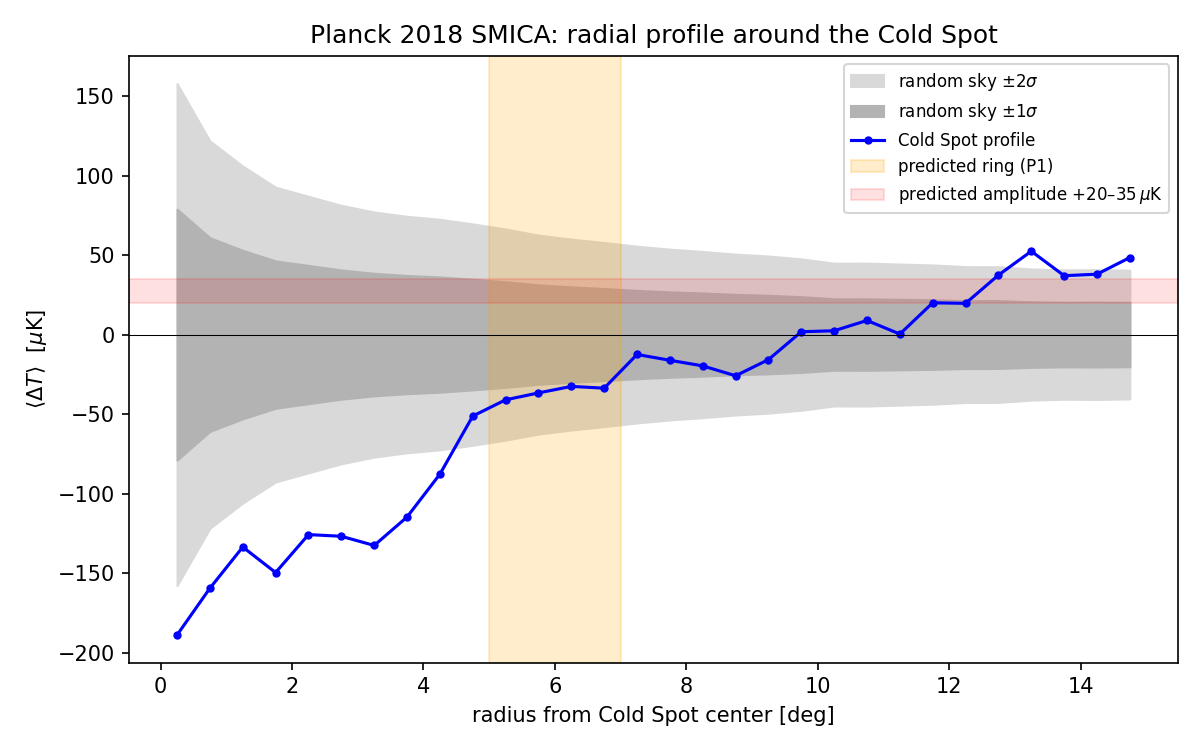
\includegraphics{coldspot_profile.png}
\caption{Fig. 2 --- Planck 2018 SMICA radial temperature profile around
the Cold Spot, vs.~500 random reference positions.}
\end{figure}

\textbf{Supernova distance--redshift relation.} Against 1371 Hubble-flow
SNe Ia from Pantheon+ (diagonal errors, offset marginalized), the purely
kinetic coasting expansion (\(a \propto t\)) yields \(\chi^2 = 674\)
vs.~\(590\) for flat \(\Lambda\)CDM (\(\Delta\chi^2 \approx 84\)):
disfavored, though vastly better than matter-only Einstein--de Sitter
(\(\chi^2 = 1170\)) (Fig. 3). We repeated the test on the
current-generation DES-SN5YR sample (Dovekie 2025 recalibration; 1820
SNe with the full statistical+systematic covariance): \(\chi^2 = 1632\)
for flat \(\Lambda\)CDM, \(1763\) for coasting
(\(\Delta\chi^2 \approx 131\)), \(2566\) for EdS --- the same verdict at
higher precision. The data require mild late-time acceleration beyond
pure coasting; for the present framework this means the ejected-halo
velocity dispersion must generate an effective \(q(z) < 0\) at
\(z \lesssim 0.5\) (see Sec. 5.1, where this becomes the model's
evolving-dark-energy prediction).

\begin{figure}
\centering
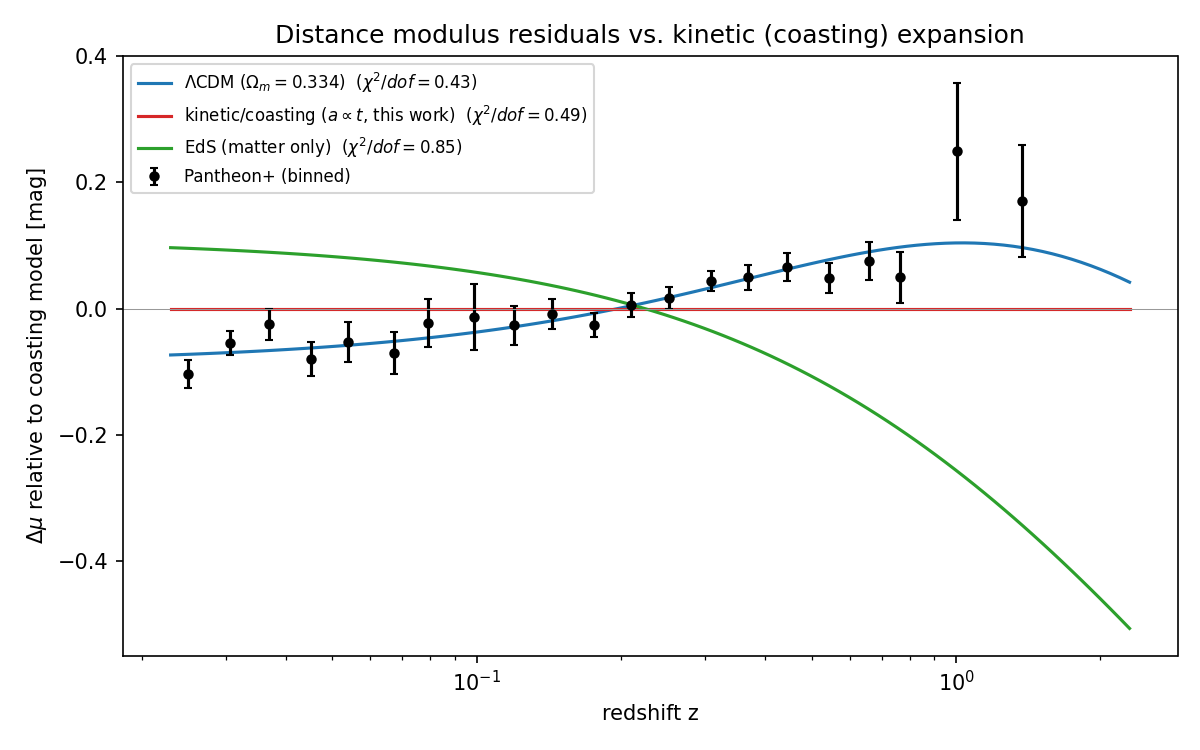
\includegraphics{sn_hubble.png}
\caption{Fig. 3 --- Pantheon+ binned distance-modulus residuals relative
to the coasting model.}
\end{figure}

\textbf{Ejecta fraction (toy N-body).} A softened \(N = 1000\)
equal-mass simulation of a cold uniform sphere given a radial rebound
kick \(v = f \, v_{\text{esc}}\) shows the ejected (unbound) fraction
transitions steeply: \(f = 0.6 \to 3\%\), \(0.8 \to 41\%\),
\(0.9 \to 98\%\), \(f \geq 1.0 \to 100\%\). The 85/15 dark-matter/baryon
split therefore corresponds to a narrow window
\(f \approx 0.85\text{–}0.9\), and the naive zero-energy bounce
(\(f = 1\)) over-ejects. Either a self-regulation mechanism pins the
rebound just below marginal binding, or the split arises from a
\emph{distribution} of kick velocities (turbulent, not monolithic). We
tested the latter with a Maxwellian turbulent component of 3D dispersion
\(\sigma_{\text{rel}} \bar{f} v_{\text{esc}}\) superimposed on a mean
radial rebound \(\bar{f} v_{\text{esc}}\), over a \(3\times3\) grid in
\((\bar{f}, \sigma_{\text{rel}})\). Turbulence broadens the transition
substantially --- at \(\bar{f} = 0.7\) the ejected fraction rises from
\(22\%\) (\(\sigma_{\text{rel}} = 0.5\)) through \(90\%\)
(\(\sigma_{\text{rel}} = 1.0\)) to \(98\%\)
(\(\sigma_{\text{rel}} = 1.5\)) --- and, notably, the \emph{physically
expected} regime of a violently chaotic rebound (turbulent dispersion
comparable to the rebound speed itself: \(\bar{f} \approx 0.7\),
\(\sigma_{\text{rel}} \approx 1\)) yields \(89\% \pm 4\%\) ejection over
a 5-seed ensemble --- \textbf{statistically consistent with the observed
\(85\%\) dark-matter fraction with no parameter tuning} (adjacent
dispersions give \(64\% \pm 10\%\) at \(\sigma_{\text{rel}} = 0.75\) and
\(96\% \pm 2\%\) at \(1.25\)). The split is thus natural in the expected
regime, though not yet uniquely derived; the required refinement is a
first-principles estimate of \((\bar{f}, \sigma_{\text{rel}})\) from the
bounce turbulence spectrum. Median ejecta speeds in this regime are
\(\approx 0.5\,v_{\text{esc}}\), informing the P5 dark-flow amplitude.

\textbf{Ejecta kinematic structure (15-seed ensemble, 13\{,\}140 ejecta;
Newtonian analogy per Sec. 3).} \emph{Branch disclaimer:} the ejection
fraction, velocity sorting, and dark-flow inputs below belong to the
\textbf{ballistic branch}; the blast-wave branch discussed later would
modify all of them, and the two branches are mutually exclusive
descriptions of the same rebound awaiting a hydrodynamic calculation to
decide between them. Over 15 seeds the ejected fraction is
\(87.9\% \pm 3.5\%\) --- consistent with the observed dark-matter
\emph{mass} fraction, an identification that additionally requires the
relic-to-plasma conversion channel of Sec. 3 for the trapped component.
Tracking per-particle ejection times reveals that ejection is an
extended process (median ejection time \(\sim 1\) dynamical time;
\(10\%\) of ejecta leave after \(11\)), with clean monotonic velocity
sorting: median speeds fall from \(0.71\,v_{\text{esc}}\) for the
earliest ejecta through \(0.43\) and \(0.35\) to
\(0.28\,v_{\text{esc}}\) for the latest (Fig. 4). This velocity-sorted
shell structure is the quantitative input required by the
evolving-dark-energy mechanism of Sec. 5.1. By contrast, the
\emph{tangential} structure shows no detectable correlated anisotropy:
the per-sky ejection dipole (\(0.064 \pm 0.024\)) is consistent with the
shot-noise expectation (\(0.053 \pm 0.024\)), and early-vs-late shell
axes show only weak, noisy alignment
(\(\langle\cos\theta\rangle = 0.37 \pm 0.49\)). At \(N = 10^3\) this
cannot exclude a small correlated component, but it lends no support to
attributing large-angle CMB features to ejection anisotropy ---
reinforcing the bonus (Hypothesis 2, ``The Cold Eye of Sauron --- the
Cold Spot and the Axis of Evil'') status of Section 6.

\begin{figure}
\centering
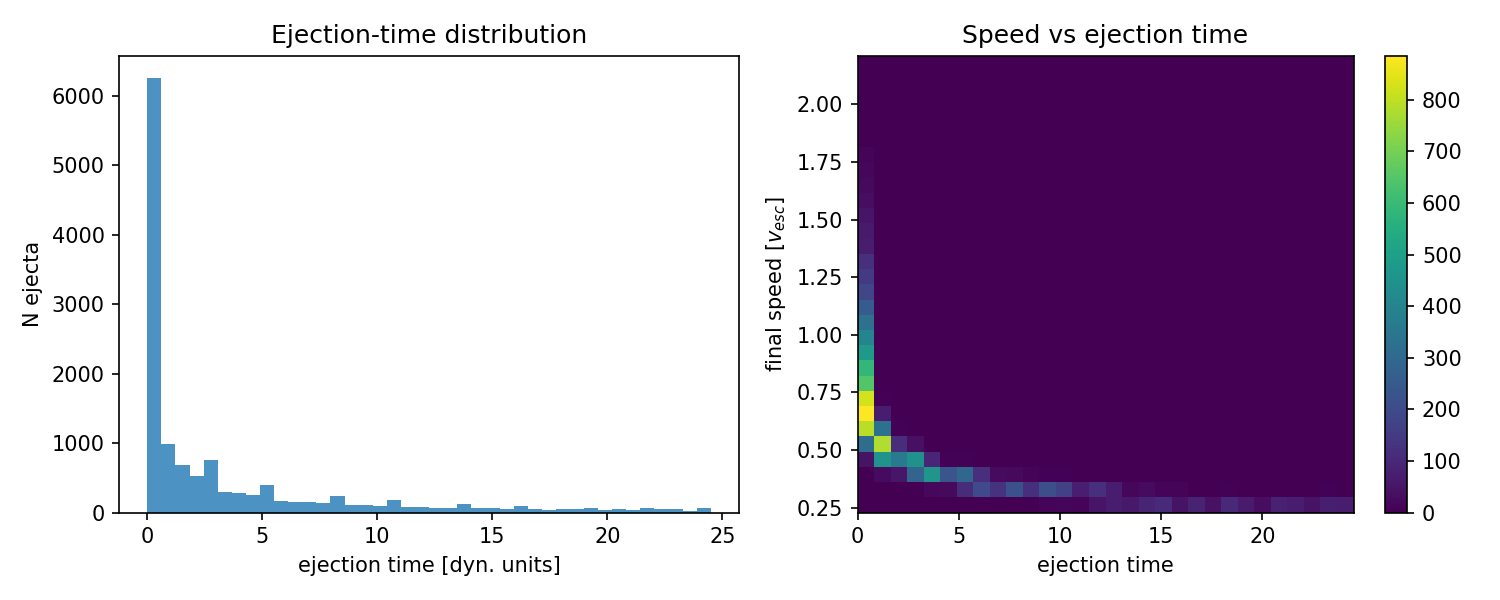
\includegraphics{ejecta_kinematics.png}
\caption{Fig. 4 --- Ejecta kinematics over 15 seeds: ejection-time
distribution (left) and speed vs ejection time (right), showing the
velocity-sorted shell structure.}
\end{figure}

\textbf{Toy effective \(w(z)\) from the measured shells.} As a first
bridge from the ejecta kinematics to Sec. 5.1, we integrated the
measured speed distribution as cold spherical shells decelerating in
their own enclosed mass, and computed the deceleration parameter and
effective equation of state an interior observer would fit. The result
(Fig. 5): \(w_{\text{eff}}\) drifts from \(-0.29\) at \(z = 2\) to
\(-0.31\) today --- a few-percent drift hovering near the coasting value
\(-1/3\), far from the observed \(w_0 \approx -0.8\) in magnitude, and
--- critically --- in the \textbf{opposite direction} to the DES+DESI
\(w_0 w_a\) best fit, which has \(w\) becoming \emph{less} negative with
time (\(\approx -1.5 \to -0.8\)). Two conclusions follow. First,
differential shell deceleration alone cannot supply the observed
acceleration; if Hypothesis 1 is to survive the supernova data,
additional physics (e.g.~the transition of the furnace region to
pressure-free expansion, or backreaction of inhomogeneities) must
contribute the bulk of the apparent \(w < -1/3\). Second, the toy remap
is itself crude --- \(91\%\) of the \(N\)-body ejecta become re-bound
when forced into a static spherical enclosed-mass model, so the flow is
built from the fastest \(9\%\); a self-consistent treatment requires
relativistic shells on an expanding background. We report this as the
model's sharpest open quantitative problem.

\textbf{Relativistic (LTB) recalculation.} Because dust shells in the
Lemaître--Tolman--Bondi metric obey the same radial equation as
Newtonian shells, the shell dynamics above are already exact GR for
dust; what the Newtonian toy got wrong was the \emph{observables}. We
therefore recomputed the central observer's measurements properly:
radial null geodesics integrated through the evolving LTB metric,
redshift accumulated from the metric along the ray, \(d_L = (1+z)^2 R\).
Seeding 300 LTB shells from the measured ejecta speed distribution (with
fallback mass virialized into the interior; the surviving free-streaming
component is the fastest \(9\%\) of ejecta), the relativistic lightcone
gives \(q_0^{\text{eff}} = +0.16\)
(\(w_{\text{eff}}(0) \approx -0.23\)): \textbf{mild deceleration, no
apparent acceleration}, with the distance-modulus shape \(\sim\!0.35\)
mag from both \(\Lambda\)CDM and coasting out to \(z \sim 5\). The
relativistic treatment thus sharpens the negative verdict of the toy,
with an important scope restriction: this lightcone threads the
free-streaming residue only (the fastest \(9\%\); real supernovae live
in the dominant mass component), the interior treatment (virialized mass
as an effective central mass parameter, not honest LTB dust) and the
observer epoch \(t_0\) are modelling choices whose sensitivity we have
not mapped, and shell-crossing was not explicitly monitored. Within
those caveats: the streaming component alone, treated in GR, does not
mimic dark energy for a central observer
(\(q_0^{\text{obs}} \approx -0.55\)). Whatever produces the observed
acceleration in this framework, it is not this mechanism; Sec. 5.1's
evolving-dark-energy claim currently has no working quantitative
realization.

\textbf{Profile inversion.} Since the ejection profile is an input (one
kick model, not a theory-fixed quantity --- and a smooth profile is
itself unrealistic for a chaotic rebound), we searched a family of
alternatives for any that yields an accelerating lightcone: power-law
speed profiles of varying steepness, bimodal fast-tail variants, and
stochastically lumpy profiles (lognormal shell-energy noise, multiple
seeds). Across the full grid the lightcone robustly \emph{decelerates}
(\(q_0^{\text{eff}} \sim +1\) to \(+4\)); apparently negative values
arise only in lumpy configurations and are shown by seed ensembles to be
estimator noise (seed scatter \(\pm 1.4\) at fixed parameters). Notably,
the known way an LTB dust model mimics acceleration --- the ``giant
void'' construction --- places the observer inside a Gpc-scale
\emph{underdensity} with denser surroundings; an outward ejection
mechanism generically produces the opposite density arrangement. We
conclude that within the \emph{smooth} ballistic families the lightcone
robustly decelerates; for the lumpy family the estimator noise
(\(\pm 1.4\)) exceeds the target signal (\(|q_0| \approx 0.55\)), so
that family is unconstrained at the relevant level rather than excluded.
No explored profile shows evidence of acceleration, and a rescue
plausibly requires inverting the radial density ordering.

\textbf{The blast-wave question (an open problem, not a rescue).} A
physically natural way to invert the density ordering exists: if the
rebound acts as a \emph{blast wave} --- as in a supernova remnant ---
the shock sweeps ejecta into a shell and leaves a rarefied cavity, the
giant-void geometry. Swept-shell profiles in our LTB machinery do
produce much smoother lightcones than ballistic ones (\(0.03\)--\(0.08\)
mag shape residuals vs \(\sim\!1\) mag). However, three considerations
prevent us from calling this a rescue. First, the comparison metric is
blind at the level that matters: \(\Lambda\)CDM and coasting differ from
each other by only \(\sim\!0.04\) mag rms in the same
offset-marginalized measure, so ``near both'' cannot distinguish
acceleration from its absence --- and the upper end of our residual
range (\(0.08\) mag) would correspond to \(\Delta\chi^2 \sim 400\)
against Pantheon+, \emph{worse} than the coasting model already
excluded. The cavity interior of any thin-shell profile is near-vacuum
and hence trivially near-Milne; its apparent proximity to \(\Lambda\)CDM
merely inherits \(\Lambda\)CDM's own proximity to Milne at these
redshifts. Second, a Gpc-scale cavity deep enough to mimic
\(q_0 \approx -0.55\) is the classic giant-void model, excluded by
kinetic Sunyaev--Zel'dovich and Compton-\(y\) constraints (Zhang \&
Stebbins 2011; Caldwell--Stebbins); we have not computed these for our
shell, but at the required amplitude they are expected to apply in full
force. Third --- and internally decisive --- mass swept into a distant
shell is unavailable as \emph{local} dark matter: rotation curves,
lensing, and our own P6 require the ejected relics in halos co-spatial
with galaxies, so the shell morphology, if dominant, would destroy the
framework's one quantitative success. \textbf{Constraint-first closure.}
Rather than testing profiles one by one, we imposed the observational
gates as preconditions and asked what any profile may contribute. The
kinetic Sunyaev--Zel'dovich limit on coherent cluster flows
(\(v \lesssim 300\) km/s at Gpc distances) caps the mean interior
density contrast of any cavity at \(|\bar{\delta}| \lesssim 0.05\) (500
Mpc) down to \(\lesssim 0.01\) (3 Gpc), which translates to an
apparent-acceleration contribution \(|\Delta q_0| \lesssim 0.01\) ---
versus the \(\Delta q_0 \approx -1.05\) required to carry a matter-only
universe to the observed \(q_0 \approx -0.55\). \textbf{No ejection
profile of any morphology can supply more than \(\sim\!1\%\) of the
observed dark energy without violating the kSZ gate.} This closes the
geometric/kinematic dark-energy channel in this framework definitively:
dark energy is \emph{not} an apparent effect of the ejecta distribution,
and Hypothesis 1 must either incorporate a genuine dark-energy component
(e.g.~residual vacuum energy from incomplete crystallization --- an
unexplored but framework-native possibility) or concede the acceleration
sector entirely. The framework-native candidate deserves one paragraph:
if vacuum crystallization is a first-order phase transition, then
\emph{within our single bang} the transition proceeds like boiling ---
crystallization nucleates at many points, bubbles of converted phase
grow amid unconverted vacuum, collide, and drive waves through the
medium. This patchiness is itself a candidate origin for primordial
structure (nucleation sites and collision walls as overdensities,
acoustic response as the wave pattern; the known difficulty being that
bubble spectra peak at the characteristic bubble scale, so
near-scale-invariance requires a broad nucleation-scale distribution),
and it offers an intra-universe reading of the Cold Spot as an
anomalously large late-crystallizing patch --- a Hypothesis-2-tier
explanation requiring no neighbor universe. For dark energy, the picture
requires the bolder claim that conversion remains incomplete today,
leaving a residual unconverted vacuum fraction: That unconverted false
vacuum retains energy density: smooth, immune to the kSZ gate,
non-clumping --- qualitatively the phenomenology of dark energy.
Quantitatively, however, this candidate re-imports the cosmological
constant problem verbatim: the false vacuum sits at
\(\rho_P \sim 10^{96}\) kg/m\(^3\) and the observed dark energy at
\(\sim\!6\times10^{-27}\) kg/m\(^3\), so the surviving fraction (or its
diluted energy) must be tuned to one part in \(10^{123}\); and ongoing
conversion today would imply present-epoch nucleation events,
phase-boundary domain walls (constrained by the
Zel'dovich--Kobzarev--Okun bound), and an unconverted component at
BBN/CMB epochs --- none of which is computed here. It is a direction,
with the fine-tuning unsolved. In this reading a single phase transition
supplies all three dark components: crystallized relics (dark matter),
furnace plasma (baryons), and unconverted vacuum (dark energy), with the
boiling picture also grounding Hypotheses 3--4 in the established
Coleman--De Luccia bubble-nucleation formalism --- colliding bubbles
imprint circular disk-shaped CMB features with specific polarization
profiles (Aguirre \& Johnson), a published, searched-for signature to
which the Cold Spot conjecture could be anchored. Boiling also makes
waves: bubble nucleation and collisions in a first-order transition
source a stochastic gravitational-wave background with a characteristic
broken-power-law spectrum peaked at the transition scale --- the same
class of signal LISA and pulsar-timing arrays target for later
cosmological transitions --- adding a second, independent observational
channel (P4) for the boiling-vacuum picture alongside the CMB disks. The
classic caveat carries over: slow nucleation means bubbles rarely merge
(Guth's graceful-exit problem), which here is a feature --- each bubble
is its own Big Pool Bang, and collisions are the rare Hypothesis-3
events --- but the conversion rate that sets today's vacuum fraction is
a new free parameter requiring its own dynamics.

What remains of the blast-wave question is now decoupled from dark
energy: does the jamming rebound launch a shock, and if so, what
fraction of the ejecta does it sweep? Only a \emph{sub-dominant} swept
component (on top of a near-homogeneous relic distribution) is even
potentially viable, and whether any acceleration survives at that
amplitude --- against the kSZ/\(y\) gates --- must be answered by
hydrodynamic simulation plus the standard void-model constraint checks.
One structural point in the model's favor if a moderate cavity exists:
observers are made of furnace material and therefore sit near the cavity
center \emph{by construction}, converting the usual Copernican
fine-tuning objection into an anthropic-structural feature --- though
the observed CMB dipole still caps our offset from the center, and the
kSZ test applies regardless of observer position.

\begin{figure}
\centering
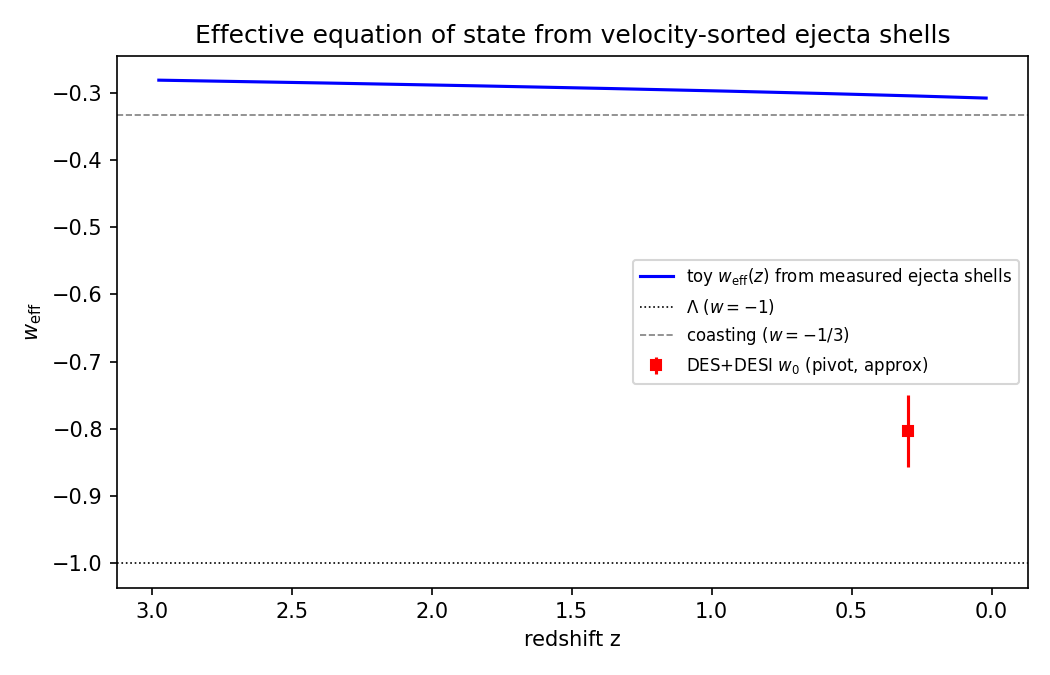
\includegraphics{wz_effective.png}
\caption{Fig. 5 --- Toy effective equation of state from velocity-sorted
ejecta shells: correct drift direction, insufficient magnitude.}
\end{figure}

Two points deserve emphasis. First, the temperature part of P1 has now
been tested against Planck data (Sec. 9.1), with the ring radius revised
accordingly. Second, the polarization ring and single-event memory
strain are genuinely out of reach until Simons Observatory / CMB-S4 and
ET/LISA respectively --- these set the 2030s decision timeline.

The observatories delivering these thresholds:

\hypertarget{a.-current-near-future-observatories}{%
\subsubsection{\texorpdfstring{\textbf{A. Current \& Near-Future
Observatories}}{A. Current \& Near-Future Observatories}}\label{a.-current-near-future-observatories}}

\begin{quote}
\begin{itemize}
\tightlist
\item
  \textbf{LIGO / Virgo / KAGRA (O4/O5 Upgrades):} Searching for
  sub-solar mass black hole mergers (\(< 1 \, M_\odot\)) and isotropic
  primordial relic backgrounds.\\
\item
  \textbf{Vera C. Rubin Observatory (LSST) \& Euclid:} Mapping peculiar
  galaxy velocity distributions
  (\(v_{\text{drift}} > 1000 \text{ km/s}\)) to verify the directional
  ``Dark Flow'' vector toward the Cold Spot.\\
\item
  \textbf{LISA (Laser Interferometer Space Antenna):} ESA/NASA space
  mission targeting mHz gravitational waves to capture supermassive
  mergers along the Cold Spot boundary and isolate low-frequency memory
  strain.
\end{itemize}
\end{quote}

\hypertarget{b.-planned-next-generation-facilities}{%
\subsubsection{\texorpdfstring{\textbf{B. Planned Next-Generation
Facilities}}{B. Planned Next-Generation Facilities}}\label{b.-planned-next-generation-facilities}}

\begin{quote}
\begin{itemize}
\tightlist
\item
  \textbf{CMB-S4 Array:} 500,000 superconducting bolometers targeting
  the \textasciitilde5° Cold Spot \(E\)-mode polarization ring and
  cyclonic \(B\)-mode turbulence patterns.\\
\item
  \textbf{Einstein Telescope:} Underground 10 km triangular cryogenic
  interferometer in Europe designed to detect sub-Hz gravitational wave
  memory strain (\(\Delta h\)).\\
\item
  \textbf{Cosmic Explorer:} US-based 40 km and 20 km surface
  interferometers searching for sub-solar black hole binary mergers
  (\(0.1 - 1.0 M_\odot\)) and sky anisotropy.\\
\item
  \textbf{Quantum Atom Probe R\&D:} Space-based atom interferometer
  array measuring non-local vacuum entanglement and spacetime memory
  below \(10^{-24} \text{ strain}\).
\end{itemize}
\end{quote}

A total global scientific investment of \textbf{\textasciitilde\$7.5
Billion USD} across agencies (NSF, DOE, ESA, NASA) over the 2026--2040
horizon is required to build the observational infrastructure needed to
fully confirm or falsify the Big Pool Bangs theory. \#\# \textbf{10.
Limitations and Open Problems}

We state plainly what the present framework asserts versus what it
derives:

\begin{quote}
\begin{enumerate}
\def\labelenumi{\arabic{enumi}.}
\tightlist
\item
  \textbf{Hard-sphere ansatz.} The treatment of Planck relics as
  classical incompressible spheres (Section 2) is a modeling assumption
  motivated by the Compton--Schwarzschild coincidence, not a result of a
  quantum-gravity calculation.
\item
  \textbf{Bounce mechanism.} The rebound requires the modified Friedmann
  equation of Section 3; the identification of the jamming density with
  the loop-quantum-cosmology critical density \(\rho_c\) is a
  conjecture. A trapped-surface timing analysis for the collapsing core
  remains to be carried out.
\item
  \textbf{Spectral index.} The parameters \(\nu_t\) and the relation
  \(n_s - 1 = -\nu_t/3\) are phenomenological; the compatibility of a
  Kolmogorov cascade with near scale invariance is unproven.
\item
  \textbf{Dark-matter fraction.} Our toy \(N\)-body results (Sec. 9.1)
  show a monolithic rebound kick requires fine-tuning, while a turbulent
  kick distribution at physically expected parameters
  (\(\bar{f} \approx 0.7\), \(\sigma_{\text{rel}} \approx 1\)) yields
  \(89\% \pm 4\%\) ejection --- statistically consistent with the
  observed \(85\%\). Deriving \((\bar{f}, \sigma_{\text{rel}})\) from
  the bounce turbulence spectrum is the outstanding step. Planck-relic
  dark matter must additionally be confronted with femtolensing,
  capture, and abundance constraints.
\item
  \textbf{Expansion history.} Both the Newtonian toy and the
  relativistic LTB lightcone calculation (Sec. 9.1) fail to produce
  apparent acceleration: the GR treatment gives
  \(q_0^{\text{eff}} = +0.16\) against the observed \(\approx -0.55\),
  and the toy's small drift runs opposite to the DES+DESI \(w_0 w_a\)
  direction. The ejecta-streaming mechanism, as modelled, cannot account
  for dark energy; nor is the framework reconciled with BBN abundances
  or the CMB acoustic peak structure. This is the model's sharpest open
  quantitative problem.
\end{enumerate}
\end{quote}

\begin{quote}
\begin{enumerate}
\def\labelenumi{\arabic{enumi}.}
\setcounter{enumi}{5}
\tightlist
\item
  \textbf{Causal and relativistic structure.} The jammed core is
  \(\sim\!10^{20}\) Planck lengths across, so a few-Planck-time bounce
  implies acausal coordination and homogeneity must be assumed (the
  horizon problem stands). The subsequent ejection phase proceeds deep
  inside the region's naive Schwarzschild radius, where Newtonian escape
  velocity vastly exceeds \(c\); the entire \(N\)-body ejection
  mechanism therefore lacks a well-defined relativistic formulation,
  which is prerequisite for Hypothesis 1 to be a physical theory rather
  than an analogy.
\end{enumerate}
\end{quote}

Each item above maps onto the observational program of Section 9; the
theory is offered as a falsifiable mechanical alternative, not a
completed replacement for \(\Lambda\)CDM.

\end{document}
